\chapter{Le quark top au LHC : production et nouvelle physique} \label{chap:new_physics}

\begin{fmffile}{chapitre5}

Le quark top est la particule élémentaire la plus lourde connue à ce jour. De par ses propriétés, le quark top doit jouer un rôle spécial dans la découverte de physique au-delà du Modèle Standard. En effet, on verra par la suite que de nombreux modèles prédisent de nouvelles particules se couplant préférentiellement au quark top. Afin d'être en mesure de mettre en évidence des couplages anormaux au quark top, il est nécessaire de bien connaître ses propriétés : c'est l'objet du début de ce chapitre.

\bigskip

Le quark top a été découvert en 1995 par les expériences \dzero et CDF au Tevatron. Son existence était cependant prédite bien avant son observation. En effet, le quark \Pbottom, découvert en 1977, se désintègre par interaction faible, désintégration autorisée uniquement lorsque la particule appartient à un doublet de $SU(2)_L$, ce qui implique qu'un partenaire d'isospin du quark \Pbottom doit exister. On présente ci-dessous les différents modes de production du quark top, ainsi que ses modes de désintégrations. Un résumé de ses propriétés sera aussi présenté.

\section{Production du quark top}

\subsection{Production par paires}

Le mécanisme de production dominant des quarks top en collisionneur hadronique se fait par interaction forte. Comme cette interaction conserve la saveur, le quark top doit être produit par paire. À \SI{14}{\TeV}, environ \SI{80}{\%} de cette production s'effectue par fusion de gluons, et \SI{20}{\%} par annihilation de quarks. Depuis peu, la section efficace de production de paire \ttbar est calculée de façon exacte au NNLO (\emph{next-to-next-to-leading order}) \citep{Czakon:2013goa}. Au LHC, pour $\sqrt{s} = \SI{8}{\TeV}$, cette section efficace a pour valeur $\sigma_{\ttbar} = \SI{245.8}{\pb}$. La \cref{fig:ttbar_diagrams} résume les diagrammes de Feynman des différents modes de production de paires \ttbar.

\begin{figure}[tbp] \centering
    \subcaptionbox{\label{fig:ttbar_fusion_gluon_1}}[0.32\textwidth]{
    \begin{fmfgraph*}(120,60)
        \fmfpen{0.5}
        \fmfleft{i1,i2}
        \fmfright{o1,o2}
        \fmf{gluon}{i1,v1,i2}
        \fmf{gluon}{v1,v2}
        \fmf{fermion}{o1,v2,o2}
        \fmfdot{v1,v2}
        \fmflabel{$t$}{o2}
        \fmflabel{$\bar{t}$}{o1}
    \end{fmfgraph*}
    }\hfill
    \subcaptionbox{\label{fig:ttbar_fusion_gluon_2}}[0.32\textwidth]{
    \begin{fmfgraph*}(140,60)
        \fmfpen{0.5}
        \fmfleft{i1,i2}
        \fmfright{o1,o2}
        \fmf{gluon}{i1,v1}
        \fmf{gluon}{i2,v2}
        \fmf{fermion}{o1,v1}
        \fmf{fermion}{v2,o2}
        \fmf{fermion,tension=1}{v1,v2}
        \fmfdot{v1,v2}
        \fmflabel{$t$}{o2}
        \fmflabel{$\bar{t}$}{o1}
    \end{fmfgraph*}
    } \hfill
    \subcaptionbox{\label{fig:ttbar_qq}}[0.32\textwidth]{
    \begin{fmfgraph*}(120,60)
        \fmfpen{0.5}
        \fmfleft{i1,i2}
        \fmfright{o1,o2}
        \fmf{fermion}{i1,v1,i2}
        \fmf{gluon}{v1,v2}
        \fmf{fermion}{o1,v2,o2}
        \fmfdot{v1,v2}
        \fmflabel{$t$}{o2}
        \fmflabel{$\bar{t}$}{o1}
    \end{fmfgraph*}
    }\hfill
    \caption{Diagrammes de Feynman de production de paires \ttbar par fusion de gluons (\subref{fig:ttbar_fusion_gluon_1}, \subref{fig:ttbar_fusion_gluon_2}), ainsi que par annihilation de quarks (\subref{fig:ttbar_qq}).}
    \label{fig:ttbar_diagrams}
\end{figure}

Lors du redémarrage du LHC en 2015 à \SI{14}{\TeV}, la section efficace de production \ttbar sera de \SI{953.6}{\pb}, soit près de 4 fois plus grande que celle à \SI{8}{\TeV}.

\subsection{Production célibataire}

Un deuxième mode de production permet de produire des quarks top célibataires, \emph{via} l'interaction faible. Trois canaux de productions existent, présentés \cref{fig:singletop_diagrams,fig:singletop_diagrams_2}. Le diagramme \cref{fig:single_top_t_channel}, connu sous le nom de voie t, est le processus dominant, avec une section efficace NNLO approchée de \SI{87.2}{\pb} au LHC à \SI{8}{\TeV} \citep{Kidonakis:2012db}. Les deux autres canaux sont la voie s (\cref{fig:single_top_s_channel}, $\sigma = \SI{5.55}{\pb}$ \citep{Kidonakis:2012db}) et la production associée d'un quark top et d'un boson \PW (voie tW, \cref{fig:singletop_diagrams_2}, $\sigma = \SI{22.2}{\pb}$ \citep{Kidonakis:2012db}). La confirmation expérimentale de ces canaux de production est très récente. En effet, le Tevatron conclut à l'existence des canaux s et t en 2009 \citep{Aaltonen:2009jj}, tandis que le canal tW a été observé pour la première fois en 2014 par l'expérience CMS \citep{Chatrchyan:1642680}.

\smallskip

Il est aussi à noter que, étant donné que le proton est chargé positivement, la production de quarks top est privilégiée face à la production de quarks anti-top. Ainsi, dans les voies s et t, la section efficace de production de quarks top est près de 2 fois plus grande que celle de production de quarks anti-top.

\begin{figure}[btp] \centering
    \subcaptionbox{\label{fig:single_top_s_channel}}[0.48\textwidth]{
    \begin{fmfgraph*}(160,70)
        \fmfpen{0.5}
        \fmfleft{i1,i2}
        \fmfright{o1,o2}
        \fmf{fermion}{i1,v1,i2}
        \fmf{boson,label=\PWplus}{v1,v2}
        \fmf{fermion}{o1,v2,o2}
        \fmfdot{v1,v2}
        \fmflabel{\Pquark}{i1}
        \fmflabel{\APquark}{i2}
        \fmflabel{\Ptop}{o2}
        \fmflabel{\APbottom}{o1}
    \end{fmfgraph*}
    }\hfill
    \subcaptionbox{\label{fig:single_top_t_channel}}[0.48\textwidth]{
    \begin{fmfgraph*}(160,70)
        \fmfpen{0.5}
        \fmfleft{i1,i2}
        \fmfright{o1,o2}
        \fmf{fermion}{i1,v1,o1}
        \fmf{fermion}{i2,v2,o2}
        \fmf{boson,label=\PWplus}{v1,v2}
        \fmfdot{v1,v2}
        \fmflabel{\Ptop}{o1}
        \fmflabel{\Pbottom}{i1}
        \fmflabel{$\Pquark^\prime$}{o2}
        \fmflabel{\Pquark}{i2}
    \end{fmfgraph*}
    }
    \caption{Diagrammes de Feynman de la production de quark top célibataire, en voie s (\subref{fig:single_top_s_channel}) et en voie t (\subref{fig:single_top_s_channel})}
    \label{fig:singletop_diagrams}
\end{figure}


\begin{figure}[tbp] \centering
    \subcaptionbox{}[0.48\textwidth]{
    \begin{fmfgraph*}(160,70)
        \fmfpen{0.5}
        \fmfleft{i1,i2}
        \fmfright{o1,o2}
        \fmf{fermion}{i1,v1}
        \fmf{fermion,label=\Pbottom}{v1,v2}
        \fmf{gluon}{i2,v1}
        \fmf{boson}{v2,o2}
        \fmf{fermion}{v2,o1}
        \fmfdot{v1,v2}
        \fmflabel{\Ptop}{o1}
        \fmflabel{\APbottom}{i1}
        \fmflabel{\PWplus}{o2}
    \end{fmfgraph*}
    }\hfill
    \subcaptionbox{}[0.48\textwidth]{
    \begin{fmfgraph*}(160,70)
        \fmfpen{0.5}
        \fmfleft{i1,i2}
        \fmfright{o1,o2}
        \fmf{fermion}{i1,v1}
        \fmf{fermion,label=$t$}{v1,v2}
        \fmf{gluon}{i2,v2}
        \fmf{boson}{v1,o1}
        \fmf{fermion}{v2,o2}
        \fmfdot{v1,v2}
        \fmflabel{$t$}{o2}
        \fmflabel{$b$}{i1}
        \fmflabel{\PWplus}{o1}
    \end{fmfgraph*}
    }
    \caption{Diagrammes de Feynman de la production associée d'un quark top célibataire et d'un boson \PW (voie tW).}
    \label{fig:singletop_diagrams_2}
\end{figure}

\section{Désintégration du quark top}

La durée de vie mesurée du quark top est d'environ $\SI{3.3e-25}{\s}$ \citep{pdg}. Ce temps de vie est suffisamment faible pour que le quark top se désintègre avant que le processus d'hadronisation ne commence ($\tau_{\text{hadronisation}} \simeq \SI{3e-24}{\s}$). Il offre donc une possibilité unique d'étudier un quark dans un état non-lié.

Le quark top se désintègre uniquement par interaction faible, selon trois modes de désintégrations : $\Ptop \rightarrow \Pbottom \PWplus$, $\Ptop \rightarrow \Pstrange \PWplus$ et $\Ptop \rightarrow \Pdown \PWplus$. La probabilité que ces désintégrations interviennent est proportionnelle aux éléments de la matrice CKM, respectivement à $\abs{V_{tb}}^2$, $\abs{V_{ts}}^2$ et $\abs{V_{td}}^2$. Le terme dominant est $\abs{V_{tb}}^2 = \num{0.89 \pm 0.07}$ \citep{pdg}. Ainsi, le quark top se désintègre majoritairement en $\Ptop \rightarrow \Pbottom \PWplus$, avec un rapport d'embranchement de $\num{0.91 \pm 0.04}$ \citep{pdg}.

L'état final exact de la désintégration du quark top dépend de la désintégration du \PW, qui se désintègre environ \SI{33}{\%} du temps en lepton - neutrino, et \SI{67}{\%} en paire de quark-antiquark. Les rapports d'embranchements exacts de la désintégration du \PW sont résumés \cref{fig:br_W}.

\begin{table}[h] \centering
    \begin{tabular}{@{}cc@{}} \toprule
      Canal & Rapport d'embranchement  \\ \midrule
      \Pe + \Pnue & \num{0.1075 \pm 0.0013} \\
      \Pmu + \Pnum & \num{0.1057 \pm .0015} \\
      \Ptau + \Pnut & \num{0.1125 \pm .0020} \\
      \Pquark\APquark & \num{0.6760 \pm .0027} \\
      \bottomrule
    \end{tabular}
    \caption{Rapports d'embranchements des différents canaux de désintégration du boson \PW \citep{pdg}.}
    \label{fig:br_W}
\end{table}

Lors d'une production par paire, les deux quarks top vont de désintégrer de façon indépendante. Le \PW ayant 4 modes de désintégrations, l'état final d'une désintégration \ttbar peut être classé en 3 catégories :

\begin{itemize}
    \item Les deux \PW se désintègrent en $\Plepton + \Pneutrino$. On parle alors de désintégration di-leptonique (canal di-lepton).
    \item Un \PW se désintègre en $\Plepton + \Pneutrino$, et le deuxième en $\Pquark\APquark$. C'est le canal semi-lepto\-ni\-que, aussi appelé lepton + jets.
    \item Finalement, les deux \PW peuvent aussi se désintégrer en $\Pquark\APquark$. On parle dans ce cas de canal tout-hadronique.
\end{itemize}

\begin{figure}[tbp]
    \centering
    \subcaptionbox{\label{fig:top_pair_decay_channels}}[0.45\textwidth]{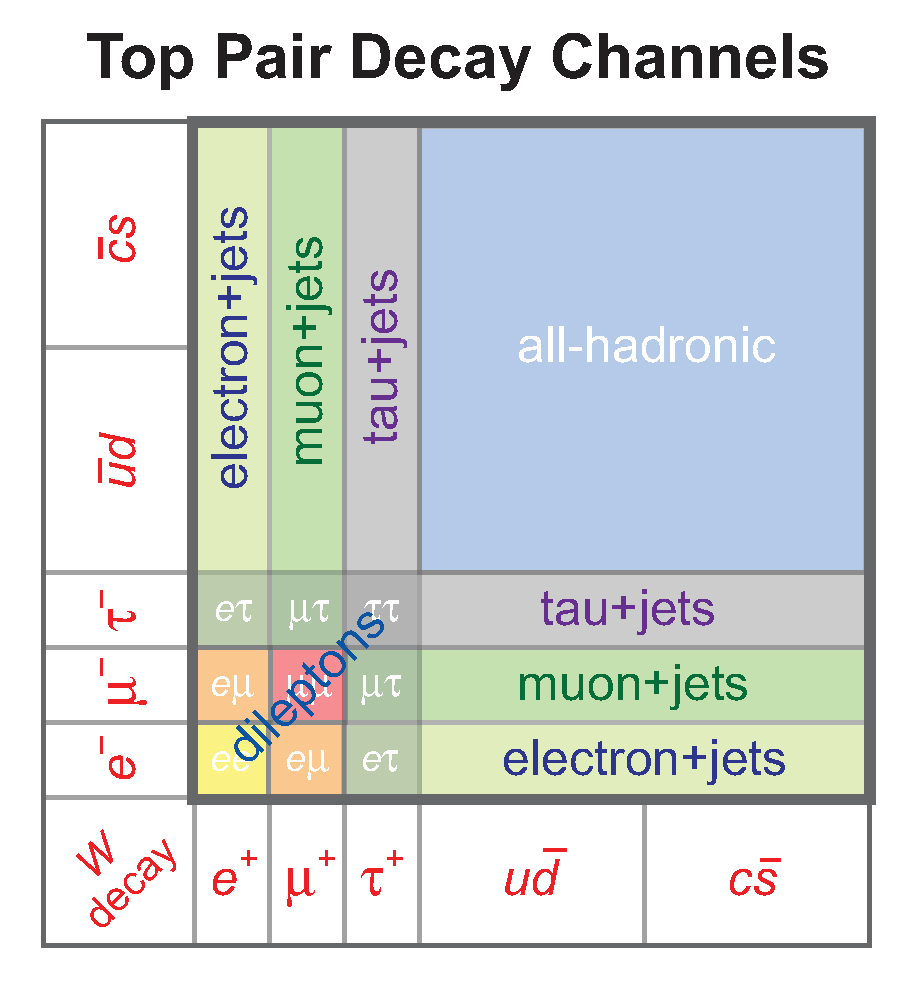
\includegraphics[width=0.40\textwidth]{chapitre5/figs/top_pair_decay_channels.pdf}} \qquad
    \subcaptionbox{\label{fig:top_pair_branching_frac}}[0.45\textwidth]{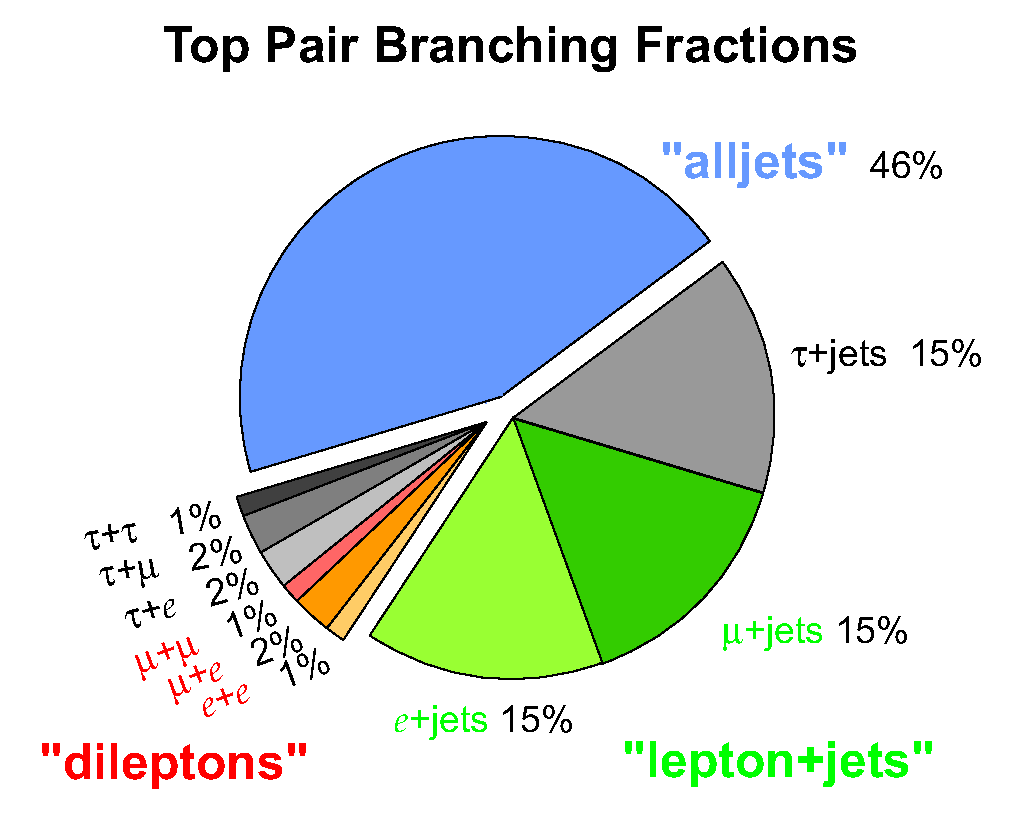
\includegraphics[width=0.45\textwidth]{chapitre5/figs/top_pair_branching_frac.pdf}}
    \caption{Canaux de désintégration d'une paire \ttbar (\subref{fig:top_pair_decay_channels}) et rapports d'embranchements des différents canaux de désintégration d'une paire \ttbar (\subref{fig:top_pair_branching_frac})}
\end{figure}

Cette classification est résumée \cref{fig:top_pair_decay_channels}. Les rapports d'embranchements associés à chaque canal de désintégration sont résumés \cref{fig:top_pair_branching_frac}. On constate ainsi qu'environ \SI{46}{\%} des paires \ttbar se désintègrent dans le canal tout-hadronique, \tilde\SI{45}{\%} dans le canal semi-leptonique, et \tilde\SI{9}{\%} dans le canal di-leptonique. Les diagrammes de Feynman associés à ces désintégrations sont présentés \cref{fig:top_pair_decay_feynman}.


\begin{figure}[p]
    \centering
    \subcaptionbox{\label{fig:top_pair_decay_dileptonic}}[0.48\textwidth]{\begin{fmfgraph*}(180,150)
        \fmfpen{0.5}
        \fmfleft{t1,i1,i2,t2}
        \fmfright{o1,o2,o3,o4,o5,o6}

        \fmf{gluon}{i1,v1,i2}
        \fmf{gluon}{v1,v2}
        \fmf{fermion,label=\APtop,label.side=left}{v3,v2}
        \fmf{fermion,label=\Ptop,label.side=left}{v2,v4}
        \fmf{boson,label=\PWplus,label.side=left}{v4,v6}
        \fmf{boson,label=\PWminus,label.side=right}{v3,v5}
        \fmf{fermion}{v5,o1}
        \fmf{fermion}{o6,v6}

        \fmffreeze

        \fmf{fermion}{o3,v3}
        \fmf{fermion}{v4,o4}

        \fmf{fermion}{v6,o5}
        \fmf{fermion}{o2,v5}

        \fmflabel{\Pleptonminus}{o1}
        \fmflabel{\APnulepton}{o2}

        \fmflabel{\APbottom}{o3}
        \fmflabel{\Pbottom}{o4}

        \fmflabel{\Pnulepton}{o5}
        \fmflabel{\Pleptonplus}{o6}

        \fmfdot{v1,v2,v3,v4,v5,v6}
    \end{fmfgraph*}}\hfill
    \subcaptionbox{\label{fig:top_pair_decay_semileptonic}}[0.48\textwidth]{\begin{fmfgraph*}(180,150)
        \fmfpen{0.5}
        \fmfleft{t1,i1,i2,t2}
        \fmfright{o1,o2,o3,o4,o5,o6}

        \fmf{gluon}{i1,v1,i2}
        \fmf{gluon}{v1,v2}
        \fmf{fermion,label=\APtop,label.side=left}{v3,v2}
        \fmf{fermion,label=\Ptop,label.side=left}{v2,v4}
        \fmf{boson,label=\PWplus,label.side=left}{v4,v6}
        \fmf{boson,label=\PWminus,label.side=right}{v3,v5}
        \fmf{fermion}{v5,o1}
        \fmf{fermion}{o6,v6}

        \fmffreeze

        \fmf{fermion}{o3,v3}
        \fmf{fermion}{v4,o4}

        \fmf{fermion}{v6,o5}
        \fmf{fermion}{o2,v5}

        \fmflabel{\Pleptonminus}{o1}
        \fmflabel{\APnulepton}{o2}

        \fmflabel{\APbottom}{o3}
        \fmflabel{\Pbottom}{o4}

        \fmflabel{\Pquark}{o5}
        \fmflabel{$\APquark^\prime$}{o6}

        \fmfdot{v1,v2,v3,v4,v5,v6}
    \end{fmfgraph*}}\\


    \subcaptionbox{\label{fig:top_pair_decay_hadronic}}[0.48\textwidth]{\fmfframe(0,50)(0,30){\begin{fmfgraph*}(180,150)
        \fmfpen{0.5}
        \fmfleft{t1,i1,i2,t2}
        \fmfright{o1,o2,o3,o4,o5,o6}
        \fmf{gluon}{i1,v1,i2}
        \fmf{gluon}{v1,v2}
        \fmf{fermion,label=\APtop,label.side=left}{v3,v2}
        \fmf{fermion,label=\Ptop,label.side=left}{v2,v4}
        \fmf{boson,label=\PWplus,label.side=left}{v4,v6}
        \fmf{boson,label=\PWminus,label.side=right}{v3,v5}
        \fmf{fermion}{v5,o1}
        \fmf{fermion}{o6,v6}
        \fmffreeze
        \fmf{fermion}{o3,v3}
        \fmf{fermion}{v4,o4}
        \fmf{fermion}{v6,o5}
        \fmf{fermion}{o2,v5}
        \fmflabel{$\Pquark^\prime$}{o1}
        \fmflabel{\APquark}{o2}
        \fmflabel{\APbottom}{o3}
        \fmflabel{\Pbottom}{o4}
        \fmflabel{\Pquark}{o5}
        \fmflabel{$\APquark^\prime$}{o6}
        \fmfdot{v1,v2,v3,v4,v5,v6}
    \end{fmfgraph*}}}
    \caption{Diagrammes de Feynman de la désintégration d'une paire \ttbar dans le canal di-leptonique (\subref{fig:top_pair_decay_dileptonic}), dans le canal semi-leptonique (\subref{fig:top_pair_decay_semileptonic}), ainsi que dans le canal tout-hadronique (\subref{fig:top_pair_decay_hadronic}).}
    \label{fig:top_pair_decay_feynman}
\end{figure}

\section{Propriétés du quark top}

Découvert en 1995, les propriétés du quark top sont encore assez méconnues. Il est donc très intéressant de les étudier précisément, puisque toutes déviations par rapport aux prédictions du Modèle Standard seraient le signe d'éventuelle nouvelle physique. Cette section présente un récapitulatif des dernières mesures expérimentales des propriétés du quark top.

\subsection{Masse}

Comme pour les autres particules du Modèle Standard, la masse du quark top est un paramètre libre. Il est néanmoins possible de prédire cette masse grâce aux corrections radiatives lors du calcul de la masse du boson \PW, à l'aide d'un ajustement global des paramètres électrofaibles du Modèle Standard. Cette masse est mesurée précisément par les expériences du LHC et du Tevatron, et est en excellent accord avec les prédictions théoriques :

\begin{align*}
  m_t^{\text{théorique}} &= 175{,}8 \substack{+2{,}7 \\ -2{,}4}\,\si{\GeV}\ \citep{ewk_fit} \\
  m_t^{\text{Tevatron}} &= 173{,}20 \pm 0{,}51\;\text{(stat.)} \pm 0{,}71\;\text{(syst.)}\;\si{\GeV}\ \citep{CDF:2013jga}\\
  m_t^{\text{LHC}} &= 173{,}29 \pm 0{,}23\;\text{(stat.)} \pm 0{,}92\;\text{(syst.)}\;\si{\GeV}\ \citep{CMS:2013sfa}\\
  m_t^{\text{LHC + Tevatron}} &= 173{,}34 \pm 0{,}27\;\text{(stat.)} \pm 0{,}71\;\text{(syst.)}\;\si{\GeV}\ \citep{ATLAS:2014wva}
\end{align*}

La \cref{fig:top_mass_combination} présente la dernière combinaison (mars 2014) des mesures de la masse du quark top effectuées par les expériences ATLAS, CDF, CMS et \dzero. C'est à ce jour la valeur la plus précise jamais mesurée, connue à moins d'\SI{1}{\GeV}.

\begin{figure}[tbp]
    \centering
    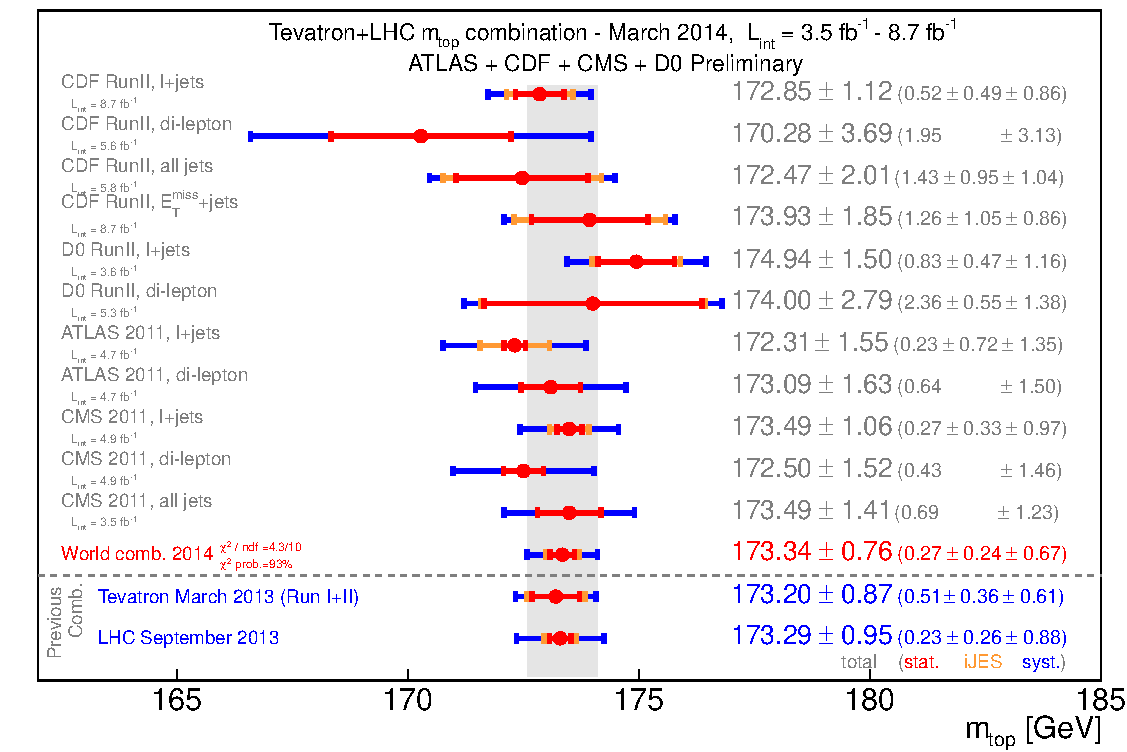
\includegraphics[width=0.70\textwidth]{chapitre5/figs/world_top_mass.pdf}
    \caption{Mesure de la masse du quark top grâce aux combinaisons des analyses ATLAS, CDF, CMS et \dzero \citep{ATLAS:2014wva}.}
    \label{fig:top_mass_combination}
\end{figure}

\subsection{Largeur}

La largeur de désintégration du quark top est prédite par le Modèle Standard. Des calculs au NLO \citep{Jezabek19891} donnent
\begin{align*}
  \Gamma_t &= \frac{G_F m_t^3}{8 \pi \sqrt{2}} \, \abs{V_{tb}}^2 \, \left( 1 - \frac{M_W^2}{m_t^2} \right)^2 \left( 1 + 2 \frac{M_W^2}{m_t^2} \right) \left[ 1 - \frac{2 \alpha_s}{3 \pi} \left( \frac{2\pi^2}{3} - \frac{5}{2} \right) \right].
\end{align*}

À l'aide de cette formule, on obtient une largeur $\Gamma_t = \SI{1.27}{\GeV}$, soit un temps de vie $\tau_t = \SI{5.16e-25}{\s}$. Expérimentalement, elle a été déterminée par les expériences \dzero et CDF au Tevatron. La valeur la plus précise obtenue à ce jour est $\Gamma_t = 2{,}00 \substack{+0{,}47 \\ -0{,}43}\,\si{\GeV}$ \citep{Abazov:2012vd}, en bon accord avec la valeur théorique.

\subsection{Charge électrique}

Rien ne permet de prouver que la particule découverte au Tevatron est bien le partenaire d'isospin du quark \Pbottom. Un modèle particulier propose en effet un quark de charge $-4/3$ et de masse \tilde \SI{170}{\GeV} comme alternative au quark top du Modèle Standard \citep{PhysRevD.59.091503}.

Afin de déterminer la charge électrique du quark top, on sélectionne des événements \ttbar dans le canal semi-leptonique. Dans le cas du modèle standard, on a
\begin{align*}
  \Ptop^{(2/3)} \rightarrow \Pbottom^{(-1/3)} + \PW^{(+1)}
\end{align*}
alors que dans le cas d'un quark top exotique ($\Ptop_X$), on a
\begin{align*}
  \Ptop_X^{(-4/3)} \rightarrow \Pbottom^{(-1/3)} + \PW^{(-1)}
\end{align*}
où la charge électrique est spécifiée entre parenthèse. En identifiant la charge du quark \Pbottom ainsi que celle du lepton (émis lors de la désintégration du boson \PWpm), il est possible de déduire la charge du quark top. Des analyses menées par les collaborations ATLAS, CDF et CMS ont permis de confirmer que la charge du quark top découvert au Tevatron est bien de charge $2/3$, avec un niveau de confiance supérieur à \SI{99}{\%} \citep{CMS-PAS-TOP-11-031,Aaltonen:2013sgl,Aad:2013uza}.


\subsection{Hélicité du boson \texorpdfstring{\PW}{W}}

Le quark top se désintègre uniquement par interaction faible, principalement en \Pbottom{}\PW. L'interaction faible ne couplant que les particules de chiralité gauche, cela limite les états d'hélicité autorisés par le Modèle Standard pour le boson \PW. En effet, au niveau de l'arbre et dans la limite d'un quark \Pbottom non massif, seuls les états d'hélicités gauche et longitudinale sont autorisés. Au NNLO, le Modèle Standard prédit les fractions d'hélicité du boson \PW suivantes \citep{Czarnecki:2010gb} :
\begin{align*}
  F_0 &= \num{0.687 \pm 0.005} \\
  F_G &= \num{0.311 \pm 0.005} \\
  F_D &= \num{0.0017 \pm 0.0001}
\end{align*}

Une déviation dans la mesure de ces fractions d'hélicités serait le signe d'un couplage \Ptop{}\PW{}\Pbottom anormal, et donc un signe de nouvelle physique. Ces fractions ont été mesurées expérimentalement par l'expérience CMS \citep{CMS-PAS-TOP-13-008}. Les valeurs obtenues,
\begin{align*}
  F_0 &= 0{,}659 \pm 0{,}015\;\text{(stat.)} \pm 0{,}023\;\text{(syst.)} \\
  F_G &= 0{,}350 \pm 0{,}010\;\text{(stat.)} \pm 0{,}024\;\text{(syst.)} \\
  F_D &= -0{,}009 \pm 0{,}006\;\text{(stat.)} \pm 0{,}020\;\text{(syst.)}
\end{align*}
sont en parfait accord avec le Modèle Standard.

\subsection{Corrélations de spin}

À cause de son temps de vie très faible, l'information de spin du quark top est directement transmise à ses produits de désintégration. La corrélation entre les spins des quarks top d'une même paire \ttbar est ainsi directement observable dans les distributions angulaires des produits de désintégration. Le Modèle Standard prédit une forte corrélation de spin \citep{PhysRevD.53.4886}, c'est-à-dire que les quarks top d'une même paire sont principalement de même hélicité, et de nombreux modèles de nouvelle physique prédisent une modification du facteur de corrélation.

\medskip

Si l'on se concentre sur la désintégration de paires \ttbar dans le canal di-leptonique, la différence entre les angles azimutaux des leptons ($\Delta\phi_{\Pleptonplus\Pleptonminus}$) est sensible à la corrélation de spin des paires \ttbar, et peut être mesurée sans reconstruire l'événement \ttbar. À l'aide de cette variable, on peut mesurer une asymétrie, définie par
\begin{align*}
  A_{\Delta\phi} &= \frac{ N\left(\Delta\phi_{\Pleptonplus\Pleptonminus} > \frac{\pi}{2} \right) - N\left(\Delta\phi_{\Pleptonplus\Pleptonminus} < \frac{\pi}{2} \right) }{ N\left(\Delta\phi_{\Pleptonplus\Pleptonminus} > \frac{\pi}{2} \right) + N\left(\Delta\phi_{\Pleptonplus\Pleptonminus} < \frac{\pi}{2} \right) },
\end{align*}
qui fournit une excellente discrimination entre une production \ttbar corrélé ou non-corrélé. Les mesures les plus récentes sont fournies par les collaborations ATLAS \citep{ATLAS:2012ao} et CMS \citep{Chatrchyan:2013wua}, qui trouvent des résultats en parfait accord avec les prédictions du Modèle Standard. Les résultats de CMS sont résumés dans le \cref{tab:top_correlation}.

\begin{table}[ht] \centering
\begin{tabular}{@{}cccc@{}} \toprule
Asymétrie & Mesure & Théorie (NLO, corrélé) & Théorie (NLO, décorrélé) \\ \midrule
$A_{\Delta\phi}$ & \num{0.113 \pm 0.017} & $0{,}115 \substack{+0{,}014 \\ -0{,}016}$ & $0{,}210 \substack{+0{,}013 \\ -0{,}008}$ \\
\bottomrule
\end{tabular}
\caption{Comparaison entre les mesures expérimentales et la théorie pour la corrélation de spin de paires \ttbar. Les mesures expérimentales indiquent la présence de corrélation de spin dans les paires \ttbar.}
\label{tab:top_correlation}
\end{table}

\section{Au-delà du Modèle Standard}

On a déjà vu lors du \cref{chap:sm} que de nombreux arguments laissent penser que le Modèle Standard n'est qu'une théorie effective d'un modèle plus fondamentale se manifestant à plus haute énergie. De nombreux modèles existent ainsi, chacun prédisant de nouvelles particules, interactions, dimensions, ... Pour autant, aucun n'a encore été confirmé expérimentalement, et nombreuses recherches sont actuellement en cours au sein des expériences du LHC afin de tenter de découvrir des signes de nouvelle physique, ou, le cas échéant, de contraindre l'espace des paramètres de ces modèles.

Parmi ces modèles, beaucoup prévoient des phénoménologies où le quark top joue un rôle particulier. En effet, étant la particule fondamentale la plus massive, il est naturel de penser que des nouvelles particules à l'échelle du \si{\TeV} se désintègrent préférentiellement en donnant au moins un quark top. Les travaux réalisés au cours de cette thèse se concentrent sur la recherche de déviations dans le spectre de masse invariante \ttbar ($\mathrm{d}\sigma / \mathrm{d}\mtt$), déviations pouvant être causées par la production résonante de paire de quark top \emph{via} la désintégration d'une particule exotique. Ces déviations peuvent se présenter sous plusieurs formes, selon la présence ou non d'interférences avec la production du Modèle Standard. Dans le cas le plus simple, elles prennent la forme d'un pic dans le spectre de masse invariante. Des structures plus complexes peuvent aussi être observées, comme la présence d'un pic suivi d'un trou. Ces déviations seront présentées plus en détails dans les \cref{chap:zprime,chap:higgs}, dédiés à la recherche expérimentale de résonances dans le spectre de masse \ttbar.

\medskip

De nombreux modèles prédisent des particules se désintégrant en paire de quark top. On présente ci-dessous une description succincte des modèles les plus prometteurs, qui ne se veut en aucun cas exhaustive. Les analyses présentées dans les prochains chapitres tentent de mettre en évidence les particules prédites par ces modèles.% On présente \cref{tab:summary_bsm} un résumé des modèles de nouvelle physique, classé selon le spin des particules prédites, leur parité sous la symétrie CP, et leur représentation sous $SU(3)_c$.

\subsection{Le Modèle Standard et les résonances \ttbar}

À la différence des autres quarks, il n'existe pas d'état lié \ttbar, son temps de vie étant trop faible devant le temps moyen d'hadronisation. La seule production résonante \ttbar prédite par le Modèle Standard se produit par la désintégration du boson de Higgs. La récente découverte d'un boson compatible avec le boson de Higgs, de masse \tilde\SI{125}{\GeV}, exclut cette possibilité puisque $m_{\PHiggs} < 2\,m_{\Ptop}$. Il n'existe donc aucune prédiction de résonance \ttbar par le Modèle Standard. Toute déviation dans le spectre de masse \ttbar serait ainsi la preuve de l'existence de nouvelle physique.

\subsection{Modèles à deux doublets de Higgs} \label{sec:2hdm}

Un seul doublet de Higgs est introduit par le Modèle Standard pour procéder à la brisure de symétrie électrofaible, mais on peut imaginer introduire plus d'un doublet. On considère plus spécifiquement dans cette section l'extension la plus simple du secteur scalaire de Higgs, où deux doublets participent à la brisure de la symétrie électrofaible, $\phi_1$ et $\phi_2$ (modèle 2HDM) \citep{Lee:1973iz,PhysRevD.15.1958,PhysRevD.18.2574}, extension nécessaire dans plusieurs modèles de nouvelle physique, tels que la supersymétrie par exemple.

\bigskip

Si l'on considère que la symétrie CP est conservée, le potentiel scalaire le plus général pour deux doublets d'hypercharge $Y = +1$, $\phi_1$ et $\phi_2$ est
\begin{align*}
  V &= m_{11}^2 \phi_1^\dagger \phi_1 + m_{22}^2 \phi_2^\dagger \phi_2 - m_{12}^2 \left( \phi_1^\dagger \phi_2 + \phi_2^\dagger \phi_1 \right) + \frac{\lambda_1}{2} \left( \phi_1^\dagger \phi_1 \right)^2 + \frac{\lambda_2}{2} \left( \phi_2^\dagger \phi_2 \right)^2 \\
    &+ \lambda_3 \phi_1^\dagger \phi_1 \phi_2^\dagger \phi_2 + \lambda_4 \phi_1^\dagger \phi_2 \phi_2^\dagger \phi_1 + \frac{\lambda_5}{2} \left[ \left(\phi_1^\dagger \phi_2 \right)^2 + \left( \phi_2^\dagger \phi_1 \right)^2\right]
\end{align*}
où $m_{ij}$ et $\lambda_i$ sont les paramètres réels de la théorie. La valeur minimale des champs $\phi_1$ et $\phi_2$ est
\begin{align*}
  \phi_1^0 &= \colvec{2}{0}{\dfrac{v_1}{\sqrt{2}}}, & \phi_2^0 &= \colvec{2}{0}{\dfrac{v_2}{\sqrt{2}}}
\end{align*}

On réexprime les champs scalaires autour de leur valeur au minimum. On trouve
\begin{align*}
  \phi_a = \colvec{2}{\phi_a^+}{\left( v_a + \rho_a + i\eta_a \right) / \sqrt{2}},\quad a = 1, 2
\end{align*}
soit 8 champs scalaires. Après brisure spontanée de la symétrie électrofaible, trois champs disparaissent pour donner la masse des bosons \PWpm et \PZz. Il reste au final cinq champs de Higgs scalaires : deux bosons chargés scalaires, \PHpm, deux bosons neutres scalaires, \PHz et \Phz, et un boson neutre pseudo-scalaire, \PAz. Les couplages des champs scalaires sont déterminés par
\begin{align*}
  \tan \beta &= \frac{v_2}{v_1},
\end{align*}
ainsi que par $\alpha$, l'angle de mélange entre \Phz et \PHz. On a en effet
\begin{align*}
 \PAz &= \eta_1 \sin \beta - \eta_2 \cos \beta \\
 \Phz &= \rho_1 \sin \alpha - \rho_2 \cos \alpha \\
 \PHz &= -\rho_1 \cos \alpha - \rho_2 \sin \alpha
\end{align*}

% Fixer la masse d'un des champs scalaires et $\tan \beta$ suffit à décrire totalement la dynamique des champs du 2HDM \fxnote{réécrire}.

\bigskip

Si l'on souhaite éviter les courants neutres changeant la saveur, fortement contraints par les mesures expérimentales, deux types de modèles sont possibles, suivant les couplages des quarks aux doublets de Higgs. Dans le modèle de type I, tous les quarks se couplent uniquement à $\phi_2$. Dans le modèle de type II, les quarks \emph{up} se couplent à $\phi_2$ et les quarks \emph{down} se couplent à $\phi_1$. Pour les deux modèles, les leptons se couplent uniquement à $\phi_2$. Les couplages des bosons scalaires neutres aux fermions sont résumés dans le \cref{tab:2hdm_couplings}.

\bigskip

À l'arbre, deux paramètres suffisent pour décrire le secteur de Higgs, et les masses des bosons \PHz et \PAz ne sont pas bornées. Dès lors qu'une de ces masses est supérieure à $2 m_{\Ptop}$, la désintégration en paires \ttbar est possible. Selon les paramètres du modèle, le rapport d'embranchement de cette désintégration peut être augmenté, et même devenir dominant voire exclusif, comme on peut le voir \cref{fig:2hdm_br}. Dans le cas d'un pseudo-scalaire, l'étude du spectre de masse invariante de paires \ttbar peut même être l'unique moyen de détection, puisque la conservation de la symétrie CP interdit la désintégration d'un pseudo-scalaire en \PWp{}\PWm{} ou \PZ{}\PZ{}.

\begin{table} \centering
    \begin{tabular}{@{}ccccccc@{}} \toprule
    & \multicolumn{3}{c}{Type I} & \multicolumn{3}{c}{Type II} \\ \midrule
    & \Phz & \PHz & \PAz & \Phz & \PHz & \PAz \\ \cmidrule{2-7}
    quarks \emph{up} & $\dfrac{\cos \alpha}{\sin \beta}$ & $\dfrac{\sin \alpha}{\sin \beta}$ & $-i \gfive \cot \beta$ & $\dfrac{\cos \alpha}{\sin \beta}$ & $\dfrac{\sin \alpha}{\sin \beta}$ & $-i \gfive \cot \beta$ \\
    quarks \emph{down} / leptons & $\dfrac{\cos \alpha}{\sin \beta}$ & $\dfrac{\sin \alpha}{\sin \beta}$ & $i \gfive \cot \beta$ & $- \dfrac{\sin \alpha}{\cos \beta}$ & $\dfrac{\cos \alpha}{\cos \beta}$  & $-i \gfive \tan \beta$ \\ \bottomrule
    \end{tabular}
    \caption{Couplage des champs scalaires neutres aux fermions, pour les modèles de type I et II.}
    \label{tab:2hdm_couplings}
\end{table}

\begin{figure}[tbp] \centering
    \subcaptionbox{\label{fig:gg_h_tt}}[0.49\textwidth]{\fmfframe(0,0)(0,50){\begin{fmfgraph*}(180,90)
        \fmfpen{0.5}
        \fmfleft{i1,i2}
        \fmfright{o1,o2}
        \fmf{gluon}{i1,v1}
        \fmf{gluon}{i2,v2}
        \fmf{fermion,tension=0.7}{v3,v1,v2,v3}
        \fmf{scalar,label=\PHz,, \PAz,label.side=left}{v3,v4}
        \fmf{fermion}{v4,o2}
        \fmf{fermion}{o1,v4}
        \fmflabel{\APtop}{o1}
        \fmflabel{\Ptop}{o2}
        \fmfdot{v1,v2,v3,v4}
        \fmfv{label=\Ptop,label.dist=20}{v3}
    \end{fmfgraph*}}}\hfill
    \subcaptionbox{\label{fig:2hdm_br}}[0.49\textwidth]{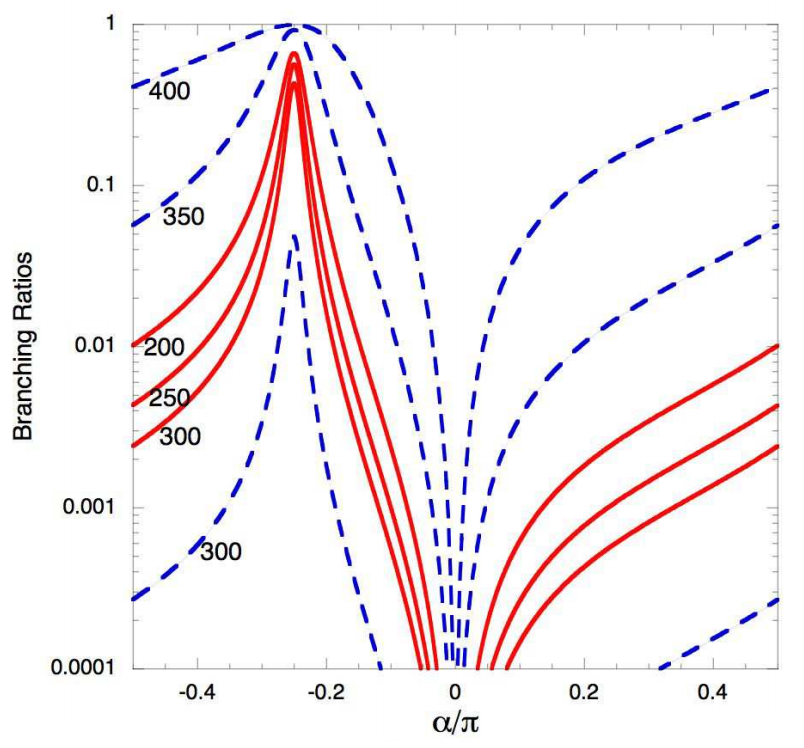
\includegraphics[width=0.49\textwidth]{chapitre5/figs/2hdm_br.png}}
    \caption{(\subref{fig:gg_h_tt}) Diagramme de Feynman de la production d'un boson scalaire neutre par fusion de gluons. (\subref{fig:2hdm_br})
    Rapport d'embranchement d'un Higgs scalaire en \bbbar (rouge) et \ttbar (bleu), pour différente masses. Les rapports d'embranchement ont été calculés pour $\tan \beta = 1$ pour le modèle de type I. \citep{Branco:2011iw}}
    \label{fig:2hdm}
\end{figure}

\begin{figure}[tbp] \centering
    \subcaptionbox{\label{fig:2hdm_mtt_scalar}}[0.49\textwidth]{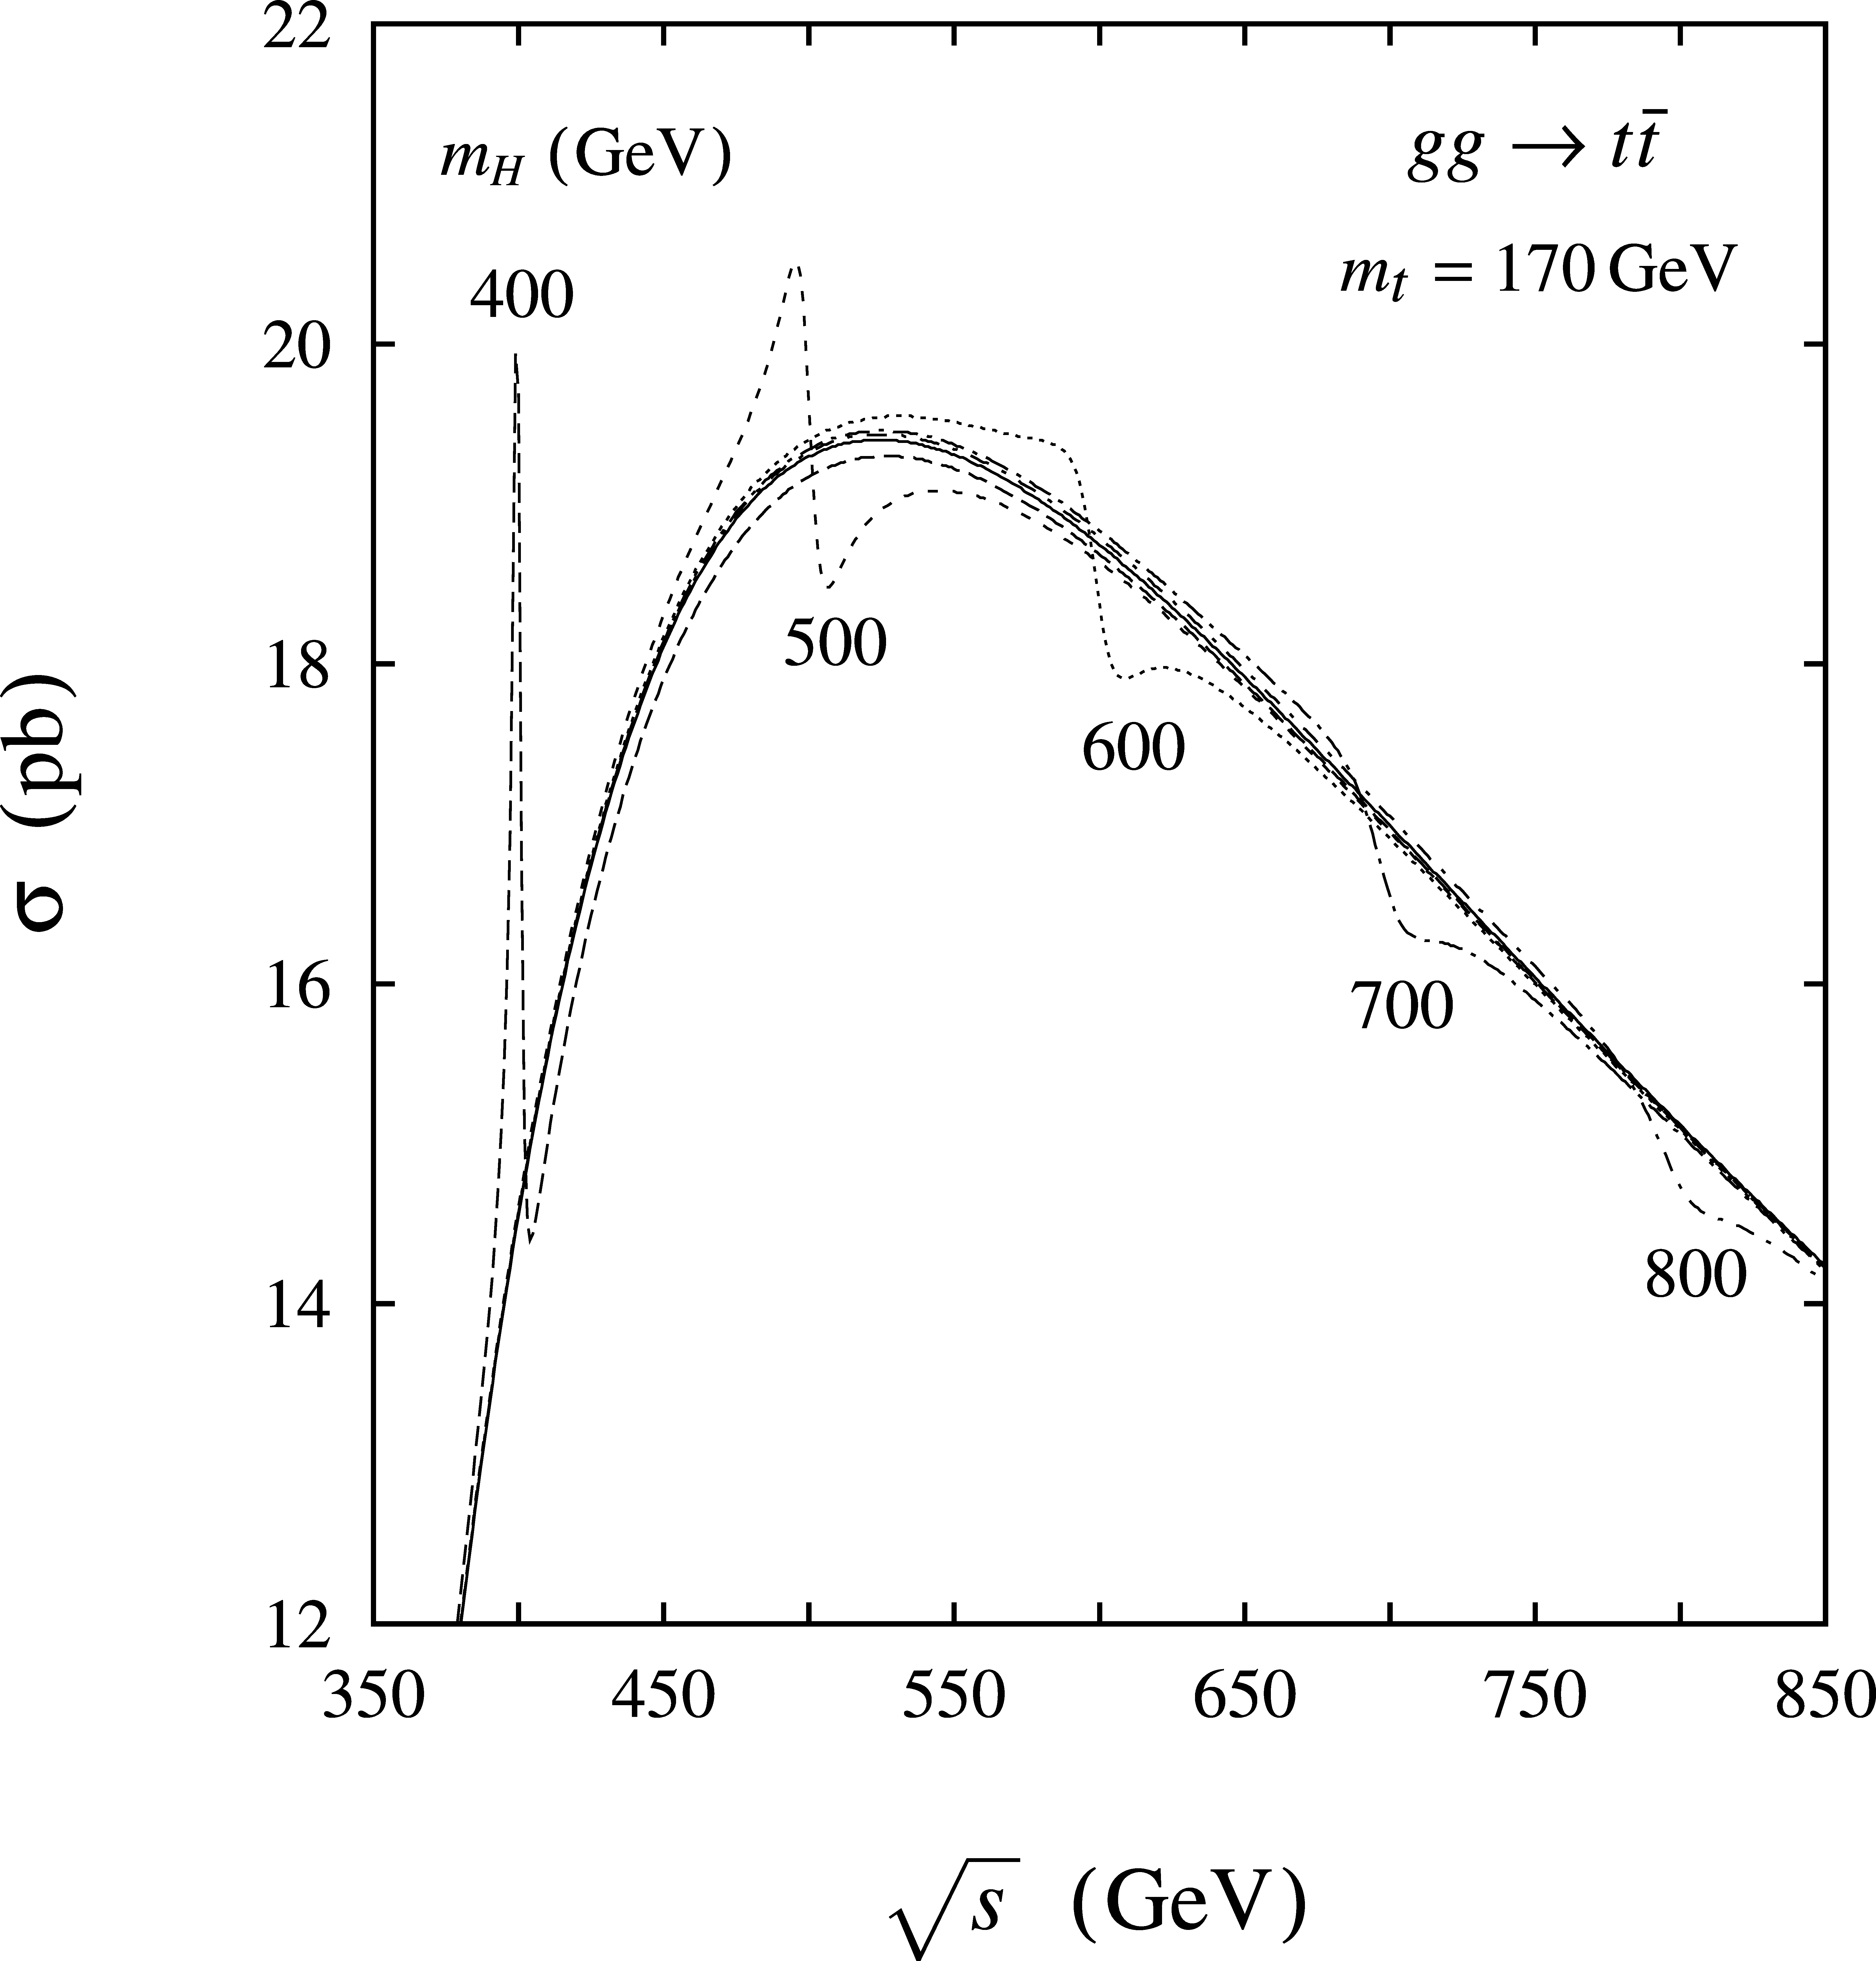
\includegraphics[width=0.49\textwidth]{chapitre5/figs/2hdm_interference.pdf}}\hfill
    \subcaptionbox{\label{fig:2hdm_mtt_pseudoscalar}}[0.49\textwidth]{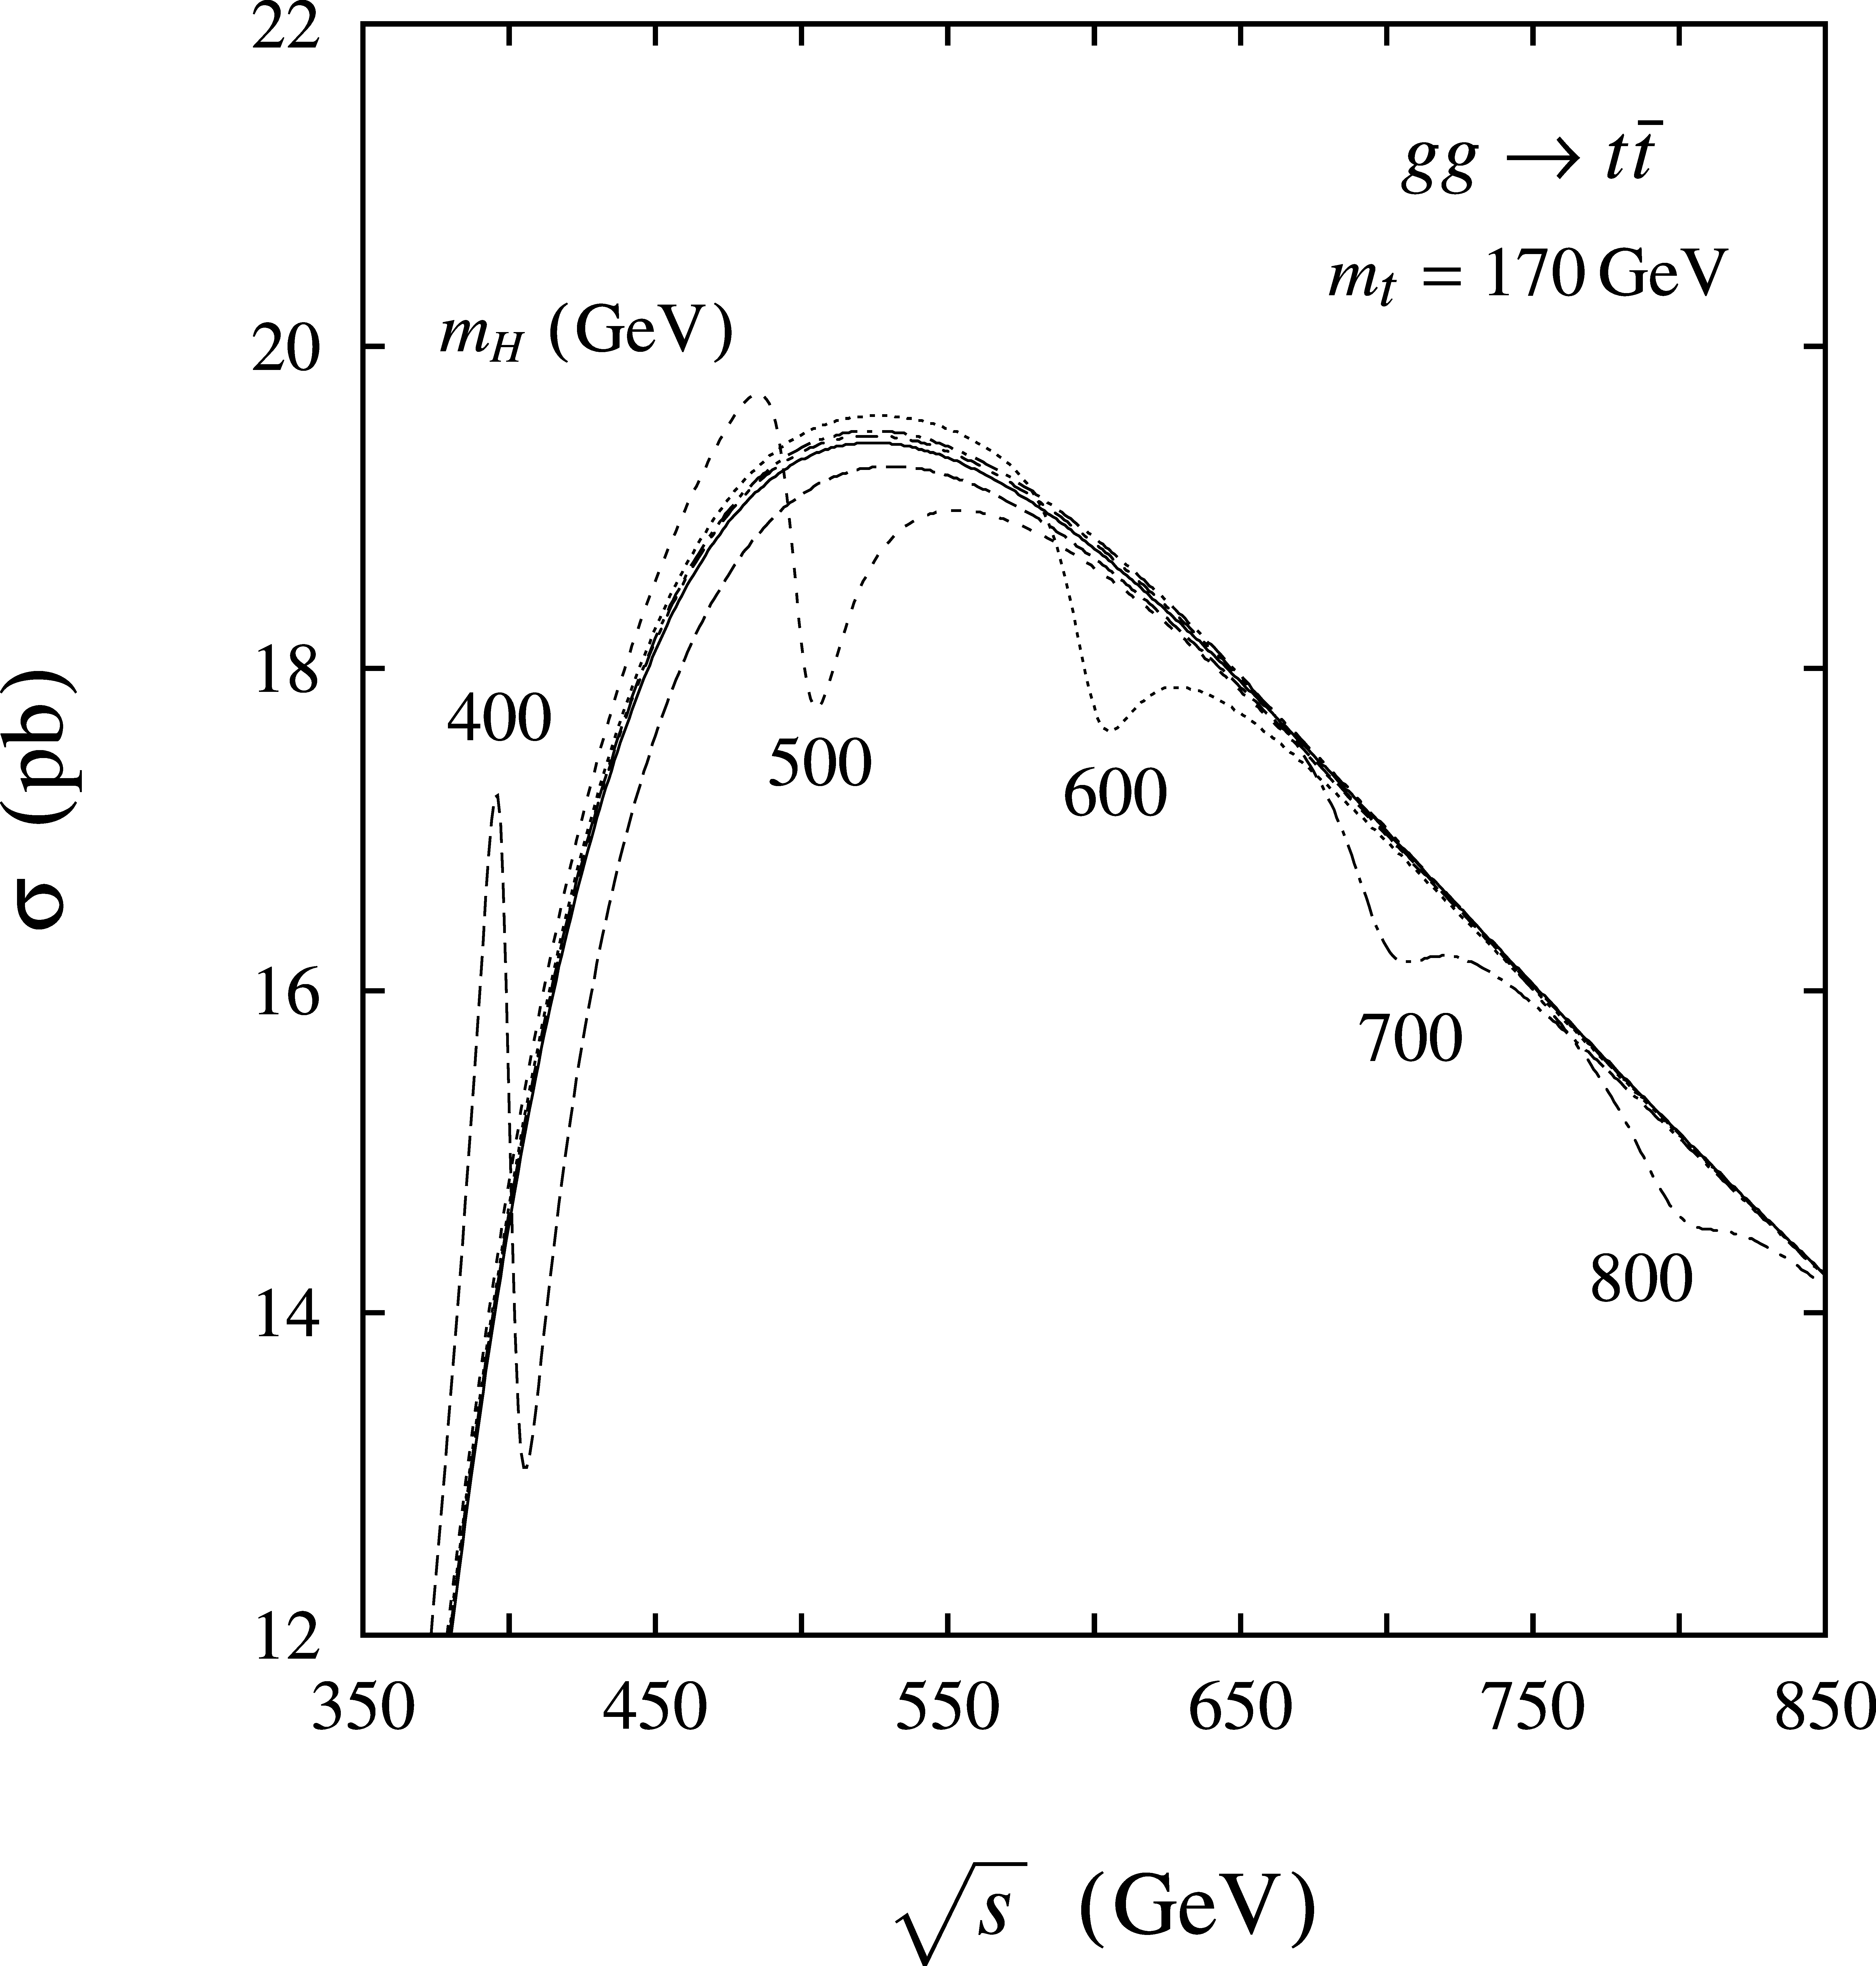
\includegraphics[width=0.49\textwidth]{chapitre5/figs/2hdm_interference_pseudoscalar.pdf}}
    \caption{Distribution de masse invariante \mtt en présence d'un boson de Higgs scalaire (\subref{fig:2hdm_mtt_scalar}) ou pseudo-scalaire (\subref{fig:2hdm_mtt_pseudoscalar}) supplémentaire se couplant à \ttbar, pour différentes masses. Les interférences avec le Modèle Standard (ligne pleine) sont clairement visibles, avec une structure pic - trou \citep{Dicus:1994bm}. Les interférences destructives sont plus marquées dans le cas d'une résonance pseudo-scalaire.}
    \label{fig:2hdm_mtt}
\end{figure}

\bigskip

Intéressons nous plus particulièrement aux bosons neutres, et plus spécifiquement à \PHz et \PAz avec une masse $m > 2 m_{\Ptop}$. Pour ces deux particules, le mode de production dominant au LHC se produit par fusion de gluon (voir \cref{fig:gg_h_tt}). L'état initial et final étant le même que le mode de production de paire \ttbar par fusion de gluon (voir \cref{fig:ttbar_fusion_gluon_1}), un phénomène d'interférence va apparaitre. En effet, l'élément de matrice $\mathcal{M}_{fi}$ intervenant dans le calcul de la section efficace (\cref{eq:section_efficace}) doit être calculé en prenant en compte les deux processus. On a donc
\begin{align*}
  \mathcal{M}_{fi} &= \mathcal{M}_{fi}^{\text{QCD}} + \mathcal{M}_{fi}^{\text{Higgs}}
\end{align*}
où $\mathcal{M}_{fi}^{\ttbar}$ est l'élément de matrice partiel du processus \Pgluon{}\Pgluon $\rightarrow$ \ttbar, et $\mathcal{M}_{fi}^{\text{Higgs}}$ l'élément de matrice partiel du processus \Pgluon{}\Pgluon $\rightarrow$ \PHz, \PAz $\rightarrow$ \ttbar. Lors de l'élévation au carré, les termes d'interférences apparaissent :
\begin{align*}
  \abs{\mathcal{M}_{fi}}^2 &= \abs{\mathcal{M}_{fi}^{\text{QCD}}}^2 + \abs{\mathcal{M}_{fi}^{\text{Higgs}}}^2 + \underbrace{\mathcal{M}_{fi}^{*\,\text{QCD}}\mathcal{M}_{fi}^{\text{Higgs}} + \mathcal{M}_{fi}^{\text{QCD}}\mathcal{M}_{fi}^{*\,\text{Higgs}}}_{\text{termes d'interférences}}
\end{align*}

Ces interférences peuvent être constructives (augmenter la section efficace) ou destructives (diminuer la section efficace) si l'élément de matrice partiel comporte une partie imaginaire. Dans le cas des bosons scalaires du modèle 2HDM, le mode de production fait intervenir une boucle de quark top virtuels, dont le couplage comporte un terme imaginaire. La résonance comportera alors une structure classique en forme de pic, où les interférences sont constructives, mais aussi un trou, où les interférences sont destructives. Cet effet particulier peut être très important, conduisant à une résonance avec une structure en pic suivi d'un trou, comme on peut le voir \cref{fig:2hdm_mtt}.

\subsection{Modèles technicolor et topcolor}

La masse des particules fondamentales est introduite par le Modèle Standard grâce au mécanisme de Higgs, détaillé lors du \cref{chap:sm}. Ce mécanisme nécessite l'introduction d'un champ scalaire qui brise la symétrie électrofaible. Les masses des particules élémentaires ne sont cependant pas prédites, et restent des paramètres libres du modèle. Ce modèle est souvent qualifié de non-naturel, dans le sens où il nécessite des ajustements fins pour garder la masse du boson de Higgs à \tilde \SI{100}{\GeV} (voir \cref{sec:sm_weakness}).

\smallskip

Le modèle technicolor \citep{PhysRevD.19.1277,PhysRevD.20.2619} évite ce problème en introduisant une nouvelle interaction de jauge similaire à celle de QCD. Le groupe de jauge considéré est dans le plupart des cas $SU(N_{T})$, ce qui revient à introduire $N_T^2 - 1$ bosons de jauges, appelés \emph{technigluons}. On introduit en plus de nouveaux fermions sans masse, les \emph{technifermions}, qui se couplent uniquement à cette nouvelle interaction. Ce choix implique donc l'existence d'une symétrie chirale $SU(N^{T}_f)_L \times SU(N^{T}_f)_R$, où $N^{T}_f$ est le nombre de saveurs des technifermions. Comme la QCD, cette interaction est asymptotiquement libre à très grande énergie, et devient forte proche de l'échelle d'énergie de la technicolor, $\Lambda_{TC} \simeq \SI{246}{\GeV}$. Il se forme alors des condensats de technifermions (\emph{technimesons} ou \emph{technibaryons}), qui brisent spontanément la symétrie chirale : les technifermions acquièrent alors dynamiquement une masse et un certain nombre de bosons de Goldstone sont créés. Si en plus ces technifermions se transforment sous $SU(2)_L \times U(1)_Y$ comme des doublets d'isopin gauche et des singlets d'isopin droit (comme les fermions du Modèle Standard), les bosons de Goldstones vont se coupler aux trois bosons médiateurs de l'interaction faible et ainsi leur donner une masse.

\smallskip

Un modèle réaliste de technicolor doit aussi pouvoir expliquer la masse des fermions. Il faut donc que les fermions du Modèle Standard se couplent aux technifermions. Le modèle de technicolor étendu \citep{Eichten1980125,Dimopoulos1979237} (ETC) étend le secteur de jauge de la technicolor afin d'ajouter des bosons de jauge massifs additionnels qui se couplent à la fois aux fermions et aux technifermions. La principale difficulté à laquelle doit faire face le modèle de technicolor étendue est la prédiction de courants neutres changeant la saveur des fermions. Un tel mécanisme est hautement supprimé dans le Modèle Standard, et les contraintes expérimentales sur de tels courants sont très importantes. Néanmoins, la technicolor étendu permet de prédire la masse de toutes les particules, mais échoue à prédire une masse élevé pour le quark top.

\medskip

Le modèle théorique topcolor \citep{Hill:1991at} a été développé dans le but d'expliquer la grande masse du quark top. Le secteur de jauge de la QCD est étendu et contenu dans un groupe de jauge $SU(3)_1 \times SU(3)_2$. L'interaction de jauge de $SU(3)_2$ couple faiblement les quarks de première et deuxième générations, alors que l'interaction de jauge de $SU(3)_1$ couple très fortement les quarks de troisième générations. La brisure $SU(3)_1 \times SU(3)_2 \rightarrow SU(3)_C$ produit un octet de bosons massifs, les \emph{topgluons}, qui se couplent principalement à $\Pbottom\APbottom$ et \ttbar. Cette interaction permet la création de condensat $\ttbar$. Le quark top acquiert alors une masse dynamique $m_t \propto \braket{\ttbar}$. Le principal problème de ce modèle est soit (1) l'échelle d'énergie se situe à très haute énergie, et la quantité d'ajustements fins nécessaire pour obtenir la masse du quark top est énorme, ou (2) l'échelle d'énergie se situe autour du \si{\TeV}, mais la masse du quark top est prédite trop grande.

\bigskip

Afin d'obtenir la masse des fermions, on considère généralement le modèle topcolor en tandem avec un autre modèle, bien souvent avec le modèle de technicolor étendu. On parle alors de "Topcolor assisted Technicolor" \citep{Hill:1994hp} (TC2, technicolor assistée par topcolor). La brisure de la symétrie électrofaible est obtenue par la technicolor. La grande masse du quark top est obtenue par une combinaison de
\begin{enumerate}
    \item Une petite composante fondamentale, $\epsilon m_{\Ptop} \ll m_{\Ptop}$, générée par ETC, de l'ordre de la masse du quark \Pbottom.
    \item Une large composante, $(1 - \epsilon)m_{\Ptop} \simeq m_{\Ptop}$, générée par la dynamique topcolor.
\end{enumerate}

Le même mécanisme s'applique aussi au quark \Pbottom. Un moyen de supprimer la création de condensat $\Pbottom\APbottom$ consiste à introduire une nouvelle interaction attractive dans le canal \ttbar et répulsive dans le canal \bbbar. On étend pour cela le secteur de jauge de l'hypercharge faible $U(1)_Y \rightarrow U(1)_{Y1} \times U(1)_{Y2}$, où $U(1)_{Y1}$ couple préférentiellement la première et deuxième générations, et $U(1)_{Y2}$ couple préférentiellement la troisième génération. La brisure de cette symétrie fait apparaitre un nouveau boson neutre de spin 1, le \zprime.

\medskip

Les topgluons et \zprime prédits par ces modèles peuvent se désintégrer en \ttbar, parfois de façon dominante. On observerait alors une résonance dans le spectre de masse \ttbar, comme on peut le voir \cref{fig:mtt_zprime}. Dans certaines configurations, il est possible d'obtenir un \zprime leptophobique \citep{Harris:1999ya} : une telle particule ne pourrait être détectée que par l'étude des paires de quark top. On peut voir \cref{fig:zprime_feynman} l'unique mode de production d'un boson \zprime au LHC. L'interférence avec la production du Modèle Standard (\cref{fig:ttbar_qq}) est très faible et peut être négligée.

\begin{figure}[tbp] \centering
    \subcaptionbox{\label{fig:zprime_feynman}}[0.39\textwidth]{\fmfframe(0,0)(0,50){\begin{fmfgraph*}(140,70)
        \fmfpen{0.5}
        \fmfleft{i1,i2}
        \fmfright{o1,o2}
        \fmf{fermion}{i1,v1,i2}
        \fmf{boson,label=\zprime,label.side=left}{v1,v2}
        \fmf{fermion}{o1,v2,o2}
        \fmflabel{\APtop}{o1}
        \fmflabel{\Ptop}{o2}
        \fmflabel{\Pquark}{i1}
        \fmflabel{\APquark}{i2}
        \fmfdot{v1,v2}
    \end{fmfgraph*}}}
    \subcaptionbox{\label{fig:mtt_zprime}}[0.60\textwidth]{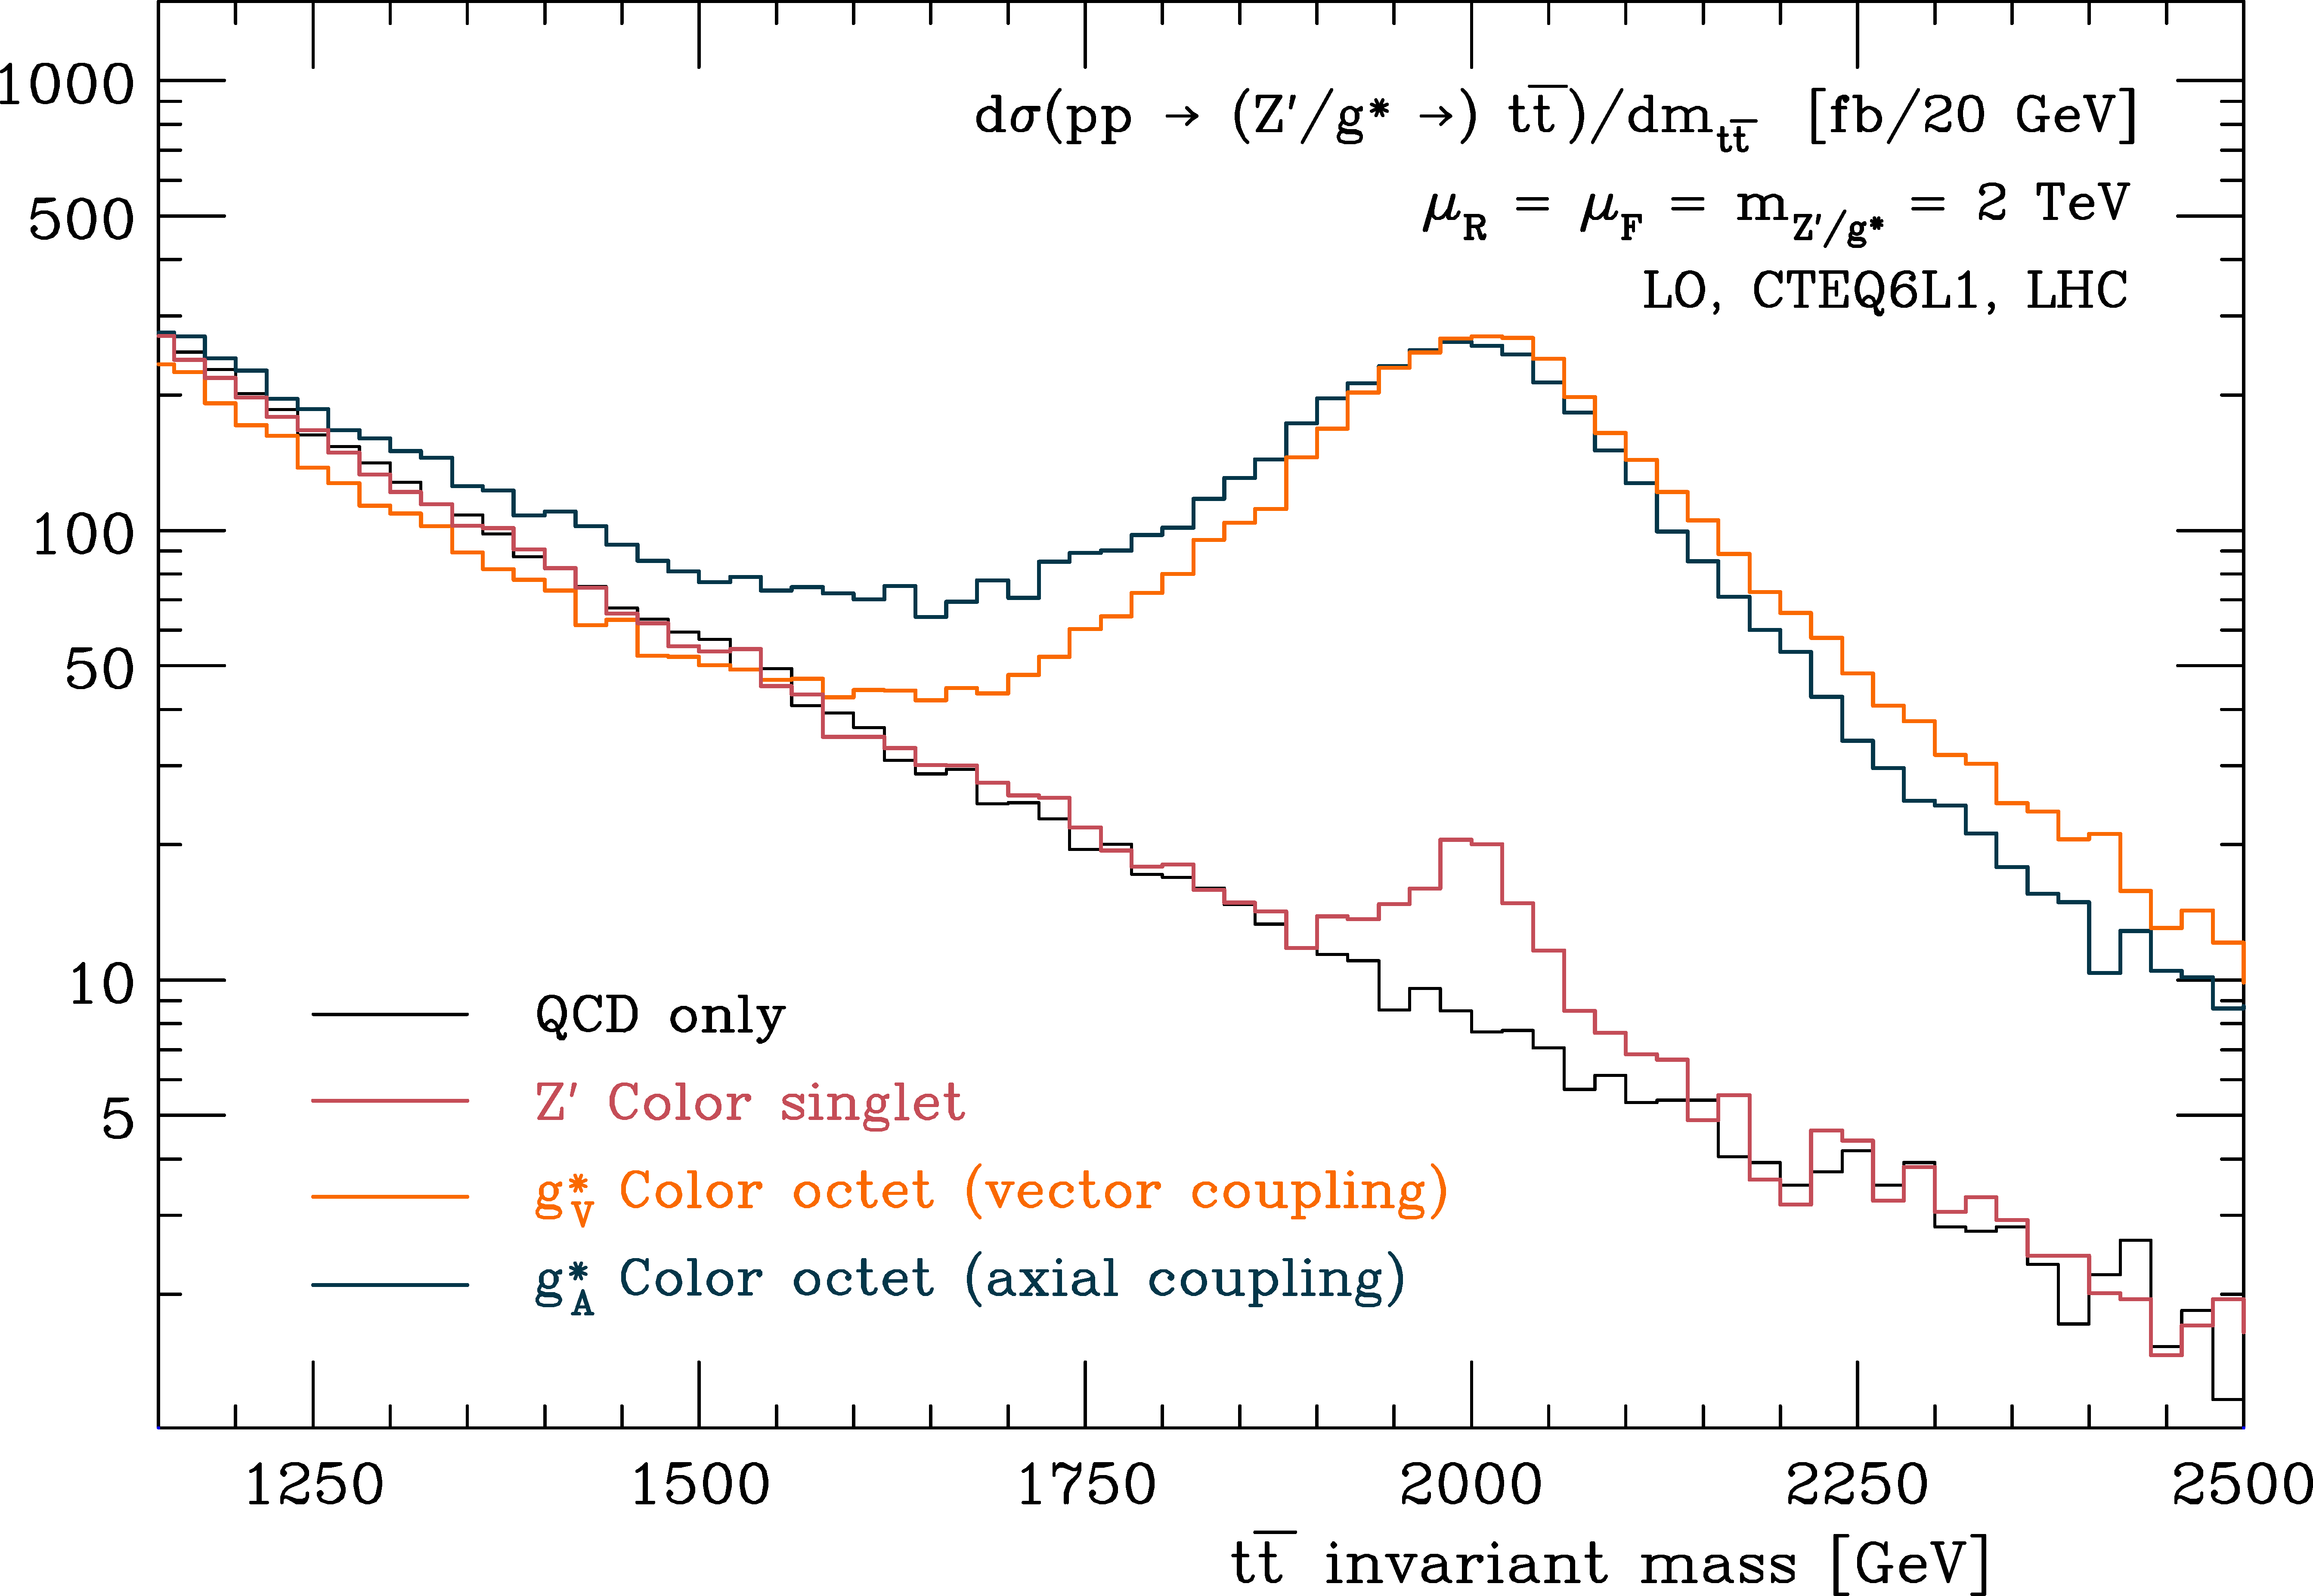
\includegraphics[width=0.60\textwidth]{chapitre5/figs/mtt_zprime.pdf}}
    \caption{(\subref{fig:zprime_feynman}) Diagramme de Feynman de la production d'un boson \zprime par annihilation de quarks. (\subref{fig:mtt_zprime}) Distribution de masse invariante \ttbar en présence de résonances de \zprime (rouge) et topgluons (bleu et orange), prédites par le modèle TC2, pour une masse $m = \SI{2}{\TeV}$ \citep{Frederix:2007gi}.}
    \label{fig:zprime}
\end{figure}

% \begin{figure}[tbp]
%     \centering
%     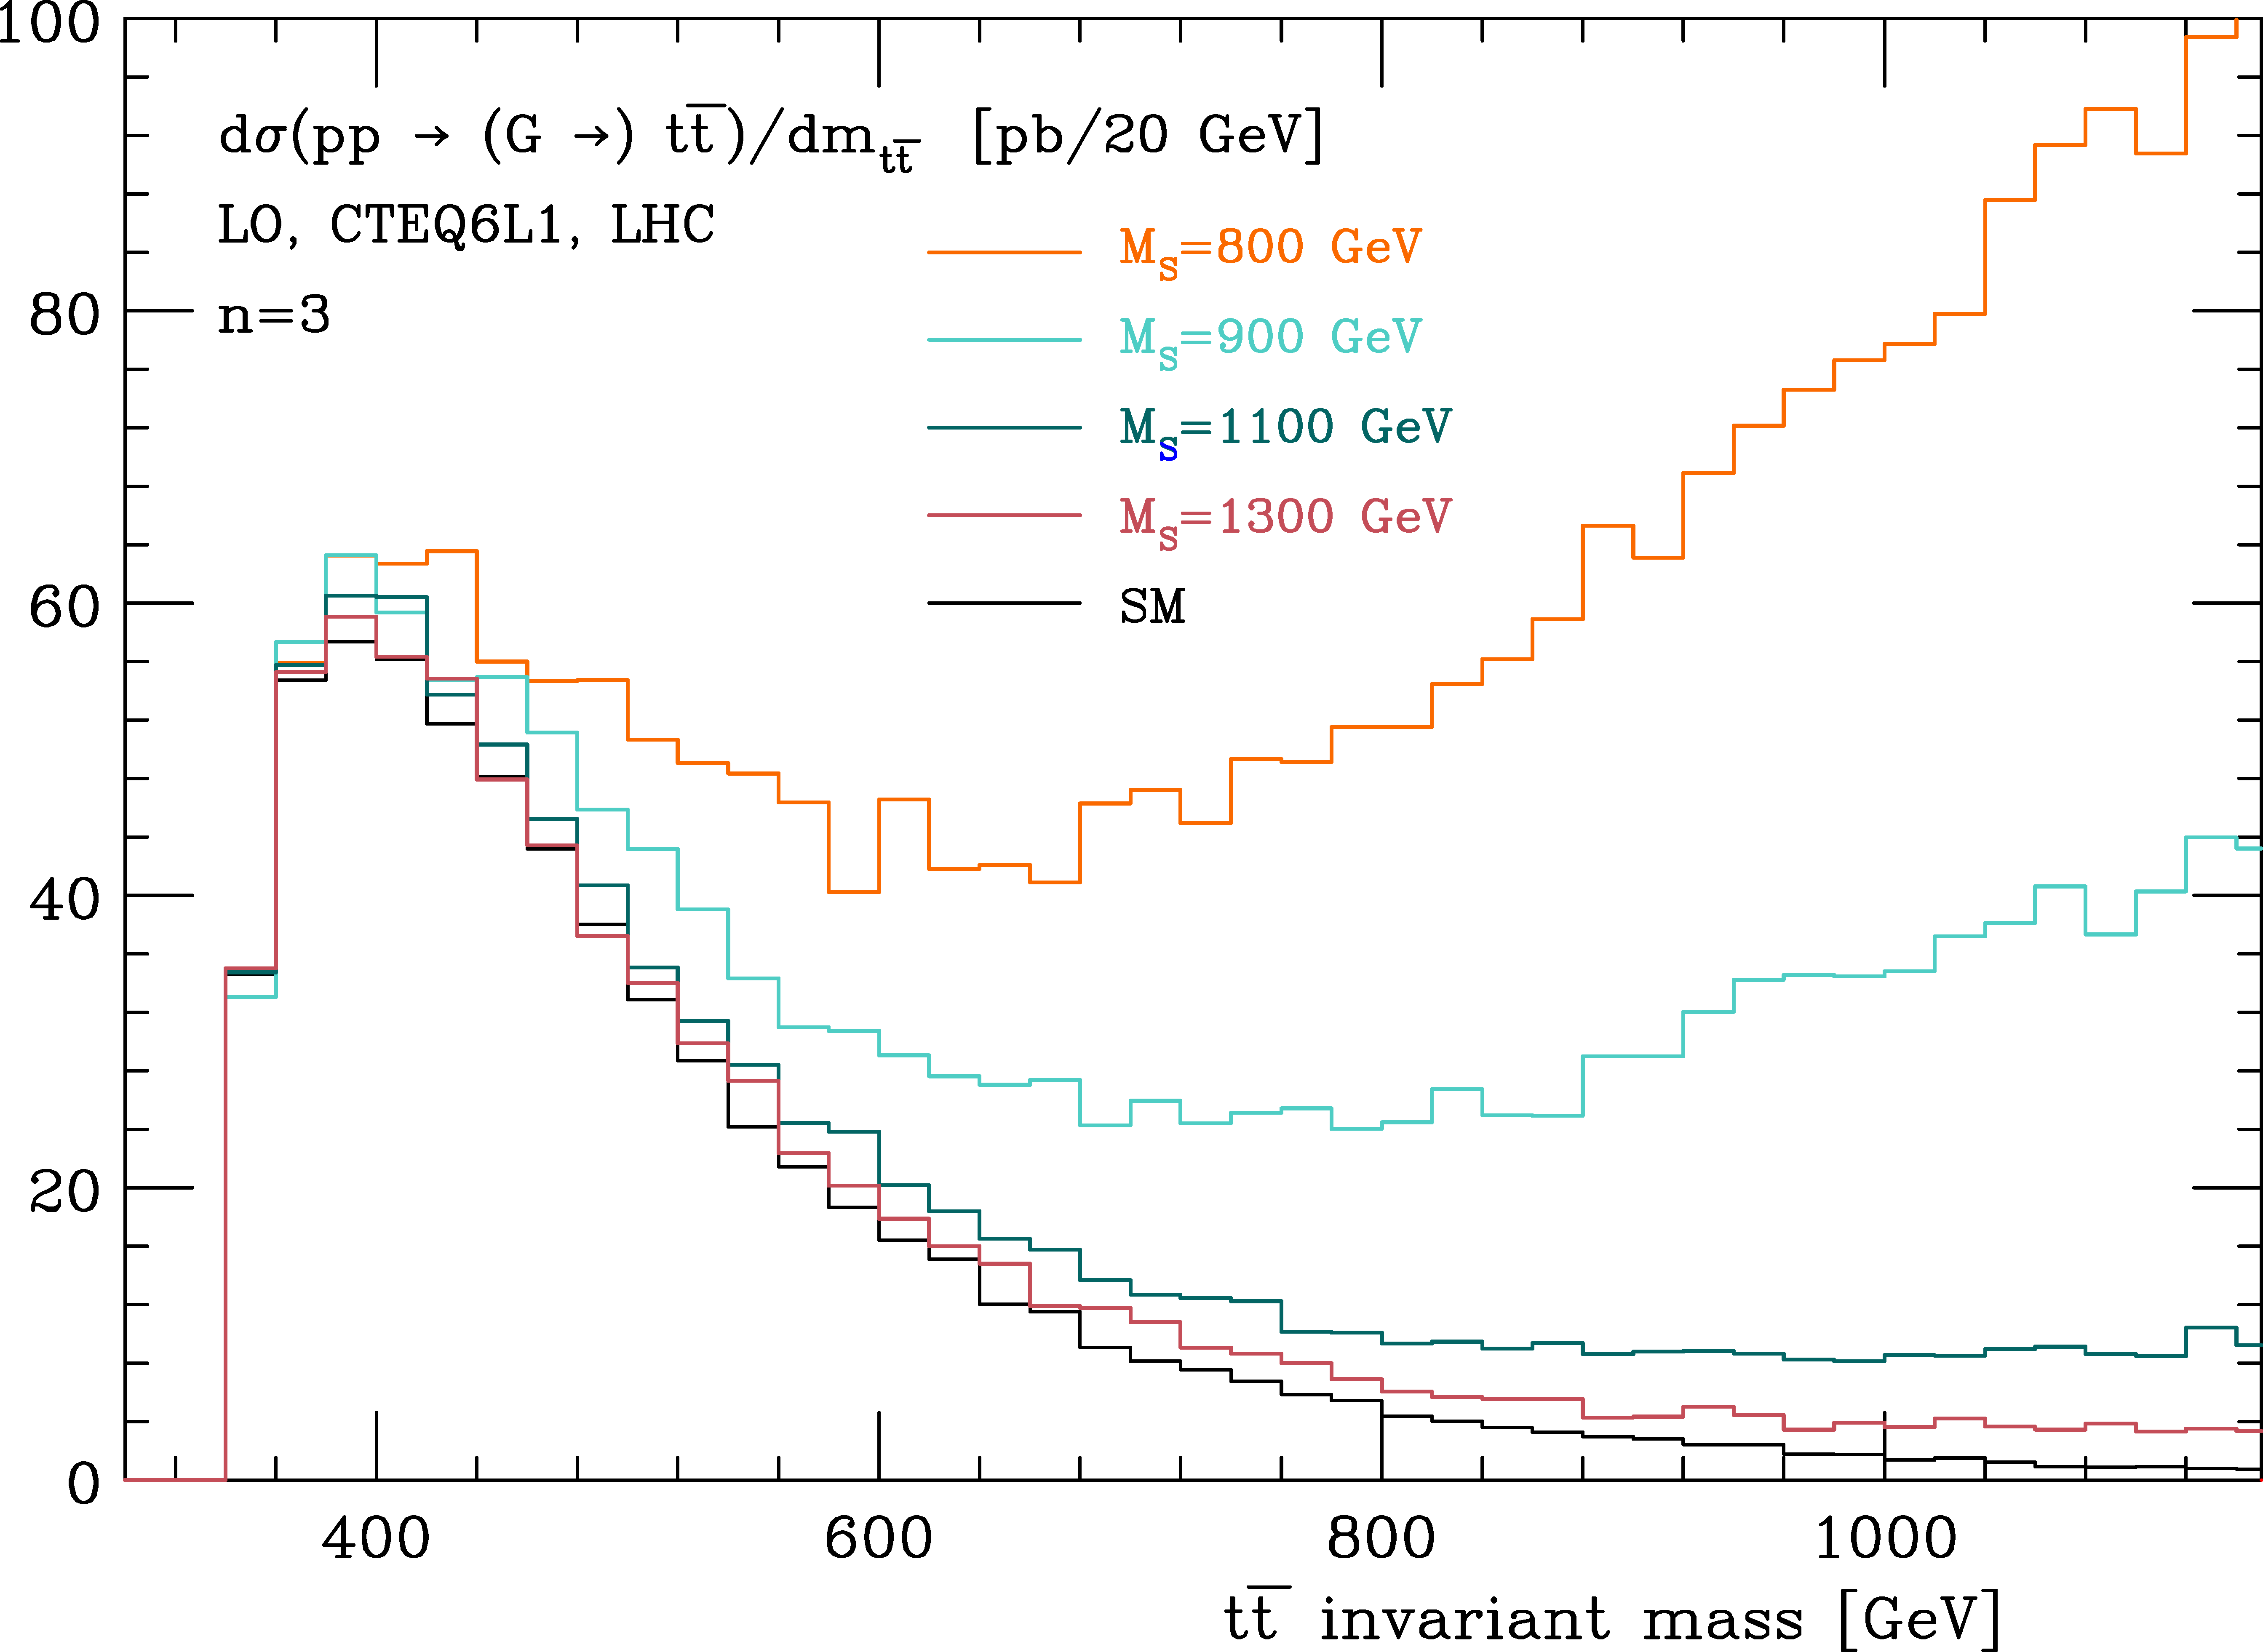
\includegraphics[width=0.60\textwidth]{chapitre5/figs/mtt_gravitons_add.pdf}
%     \caption{caption}
%     \label{fig:label}
% \end{figure}

\subsection{Modèles à dimensions supplémentaires}

Les modèles à dimensions supplémentaires ont principalement été développé afin de fournir une explication au problème de hiérarchie du Modèle Standard. En effet, l’interaction gravitationnelle est \SI{e32} fois plus faible que l'interaction faible. Dans le but d'expliquer cette différence de couplage, on introduit une ou plusieurs dimensions supplémentaire, dans lesquelles la gravitation est beaucoup plus forte que dans les dimensions usuelles de l'espace-temps. Tous ces modèles prédisent de nouveaux bosons de spin 2, les gravitons, médiateurs de l'interaction gravitationnelle.

%\subsubsection{Les modèles Randall-Sundrum}

\bigskip

\begin{figure}[tbp]
    \centering
    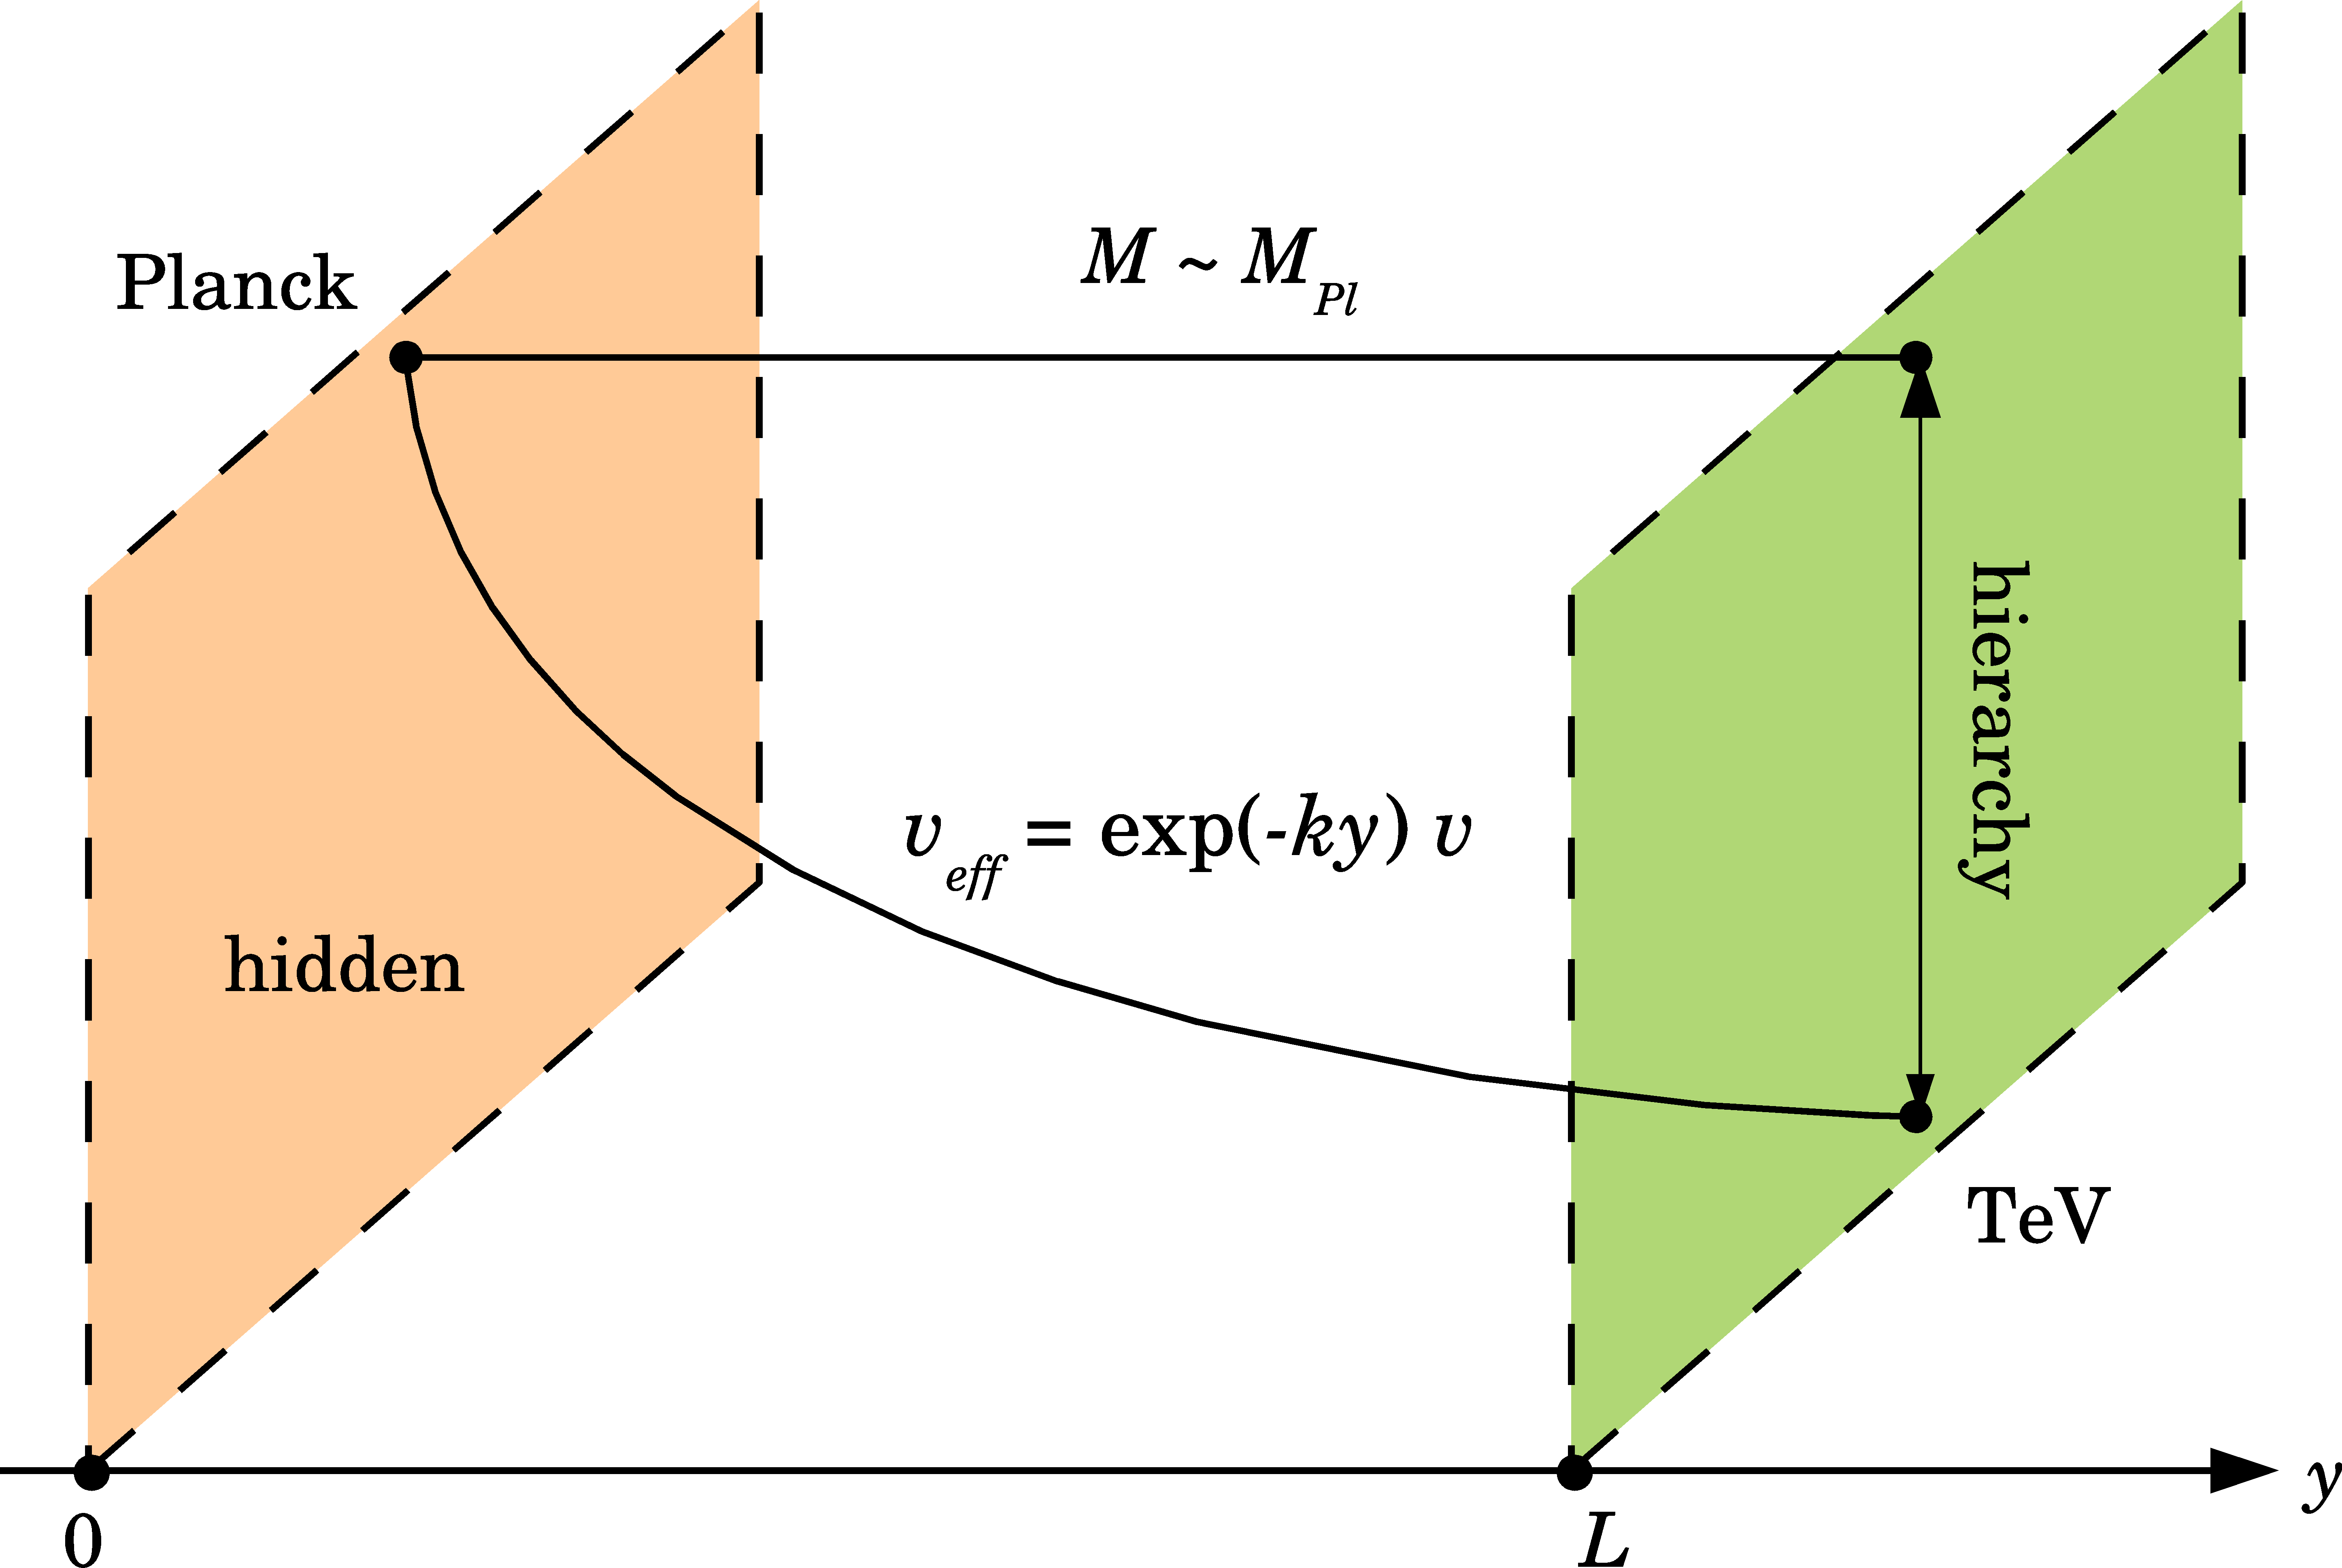
\includegraphics[width=0.6\textwidth]{chapitre5/figs/RS/hierarchie.pdf}
    \caption{Illustration de la génération du problème de hiérarchie. La brane \si{\TeV} est ici positionnée à $y = L = \pi R$.}
    \label{fig:hierarchie}
\end{figure}

Concentrons nous sur un type particulier de modèles, les modèles Randall-Sundrum. Ces modèles ajoutent une dimension supplémentaire finie aux quatre dimensions de l'espace temps \citep{Randall:1999ee,Randall:1999vf}. Cette dimension est repliée sur elle même, et elle est limitée par deux branes. La métrique est donnée par
\begin{align*}
  \mathrm{d}s^2 &= e^{-2 \kappa \abs{y}} \eta_{\mu\nu} \mathrm{d}x^\mu \mathrm{d}x^\nu + \mathrm{d}y^2
\end{align*}
où $\kappa$ est la courbure de l'espace anti de Sitter $AdS_5$, $y$ est la coordonnée dans la dimension supplémentaire, bornée par le rayon de compactification $R$ de cette dimension ($- \pi R \leq y \leq \pi R$), $\eta_{\mu\nu}$ le tenseur métrique et $x^\mu$ les coordonnées des quatre dimensions usuelles. La dimension supplémentaire est confinée entre deux 3-branes (brane à 3 dimensions), localisées à $y = 0$ et $y = \pm \pi R$, et seuls le graviton et le champ de Higgs peuvent se propager dans la cinquième dimension.

\smallskip

En introduisant une nouvelle dimension, la valeur au minimum $v$ du champ de Higgs est supprimée exponentiellement : le couplage ressenti dans notre brane n'est ainsi qu'un couplage effectif :
\begin{align*}
  v_{\text{eff}} &= e^{- \kappa \abs{y}} \, v
\end{align*}

Les masses des particules dans le Modèle Standard étant proportionnelles à $v$, on observe ainsi une suppression exponentielle de toutes les masses, expliquant ainsi le problème de hiérarchie. La \cref{fig:hierarchie} illustre cet effet : une valeur $\kappa R \simeq 11$ est suffisante pour générer la hiérarchie entre l’interaction gravitationnelle et l'interaction faible. La brane localisée à $y = 0$ est communément appelée "brane de Planck". Le couplage de l'interaction gravitationnelle y est comparable au couplage de l'interaction faible, et les particules se propageant dans cette brane ont typiquement des masses de l'ordre de la masse de Planck. Au contraire, la brane localisée à $y = \pm \pi R$ est appelée "brane \si{\TeV}" : la gravité y est très faible, et c'est ici que sont localisées les particules du Modèle Standard.

% Le problème de hiérarchie est expliqué par la fonction exponentielle, qui dépend du rayon de compactification, présente devant la métrique de l'espace à 4 dimensions usuel. Ainsi, un petit rayon de compactification peut entrainer d'énorme différentes entre l'échelle de Planck et l'échelle électrofaible. Un facteur $\kappa R \simeq 10$ permet en effet de retrouver la hiérarchie entre l'échelle de Planck et l'échelle électrofaible.

\medskip

La dimension supplémentaire étant compactifiée, on voit apparaitre des excitations de Kaluza-Klein du graviton, dont la masse $m_n$ de la $\text{n}^\text{e}$ excitation est donnée par $m_n = x_n \kappa e^{-\pi \kappa R}$, avec $x_n$ la valeur du $\text{n}^\text{e}$ zéro de la fonction de Bessel $J_1(x)$ \citep{Davoudiasl:2000wi}. Le graviton se couplant préférentiellement à la masse, la désintégration en paire \ttbar est dominante : chaque mode d'excitation apparait alors comme une résonance dans le spectre de masse \ttbar, comme on peut le voir \cref{fig:mtt_gravitons_RS}.

\bigskip

\begin{figure}[tbp]
    \centering
    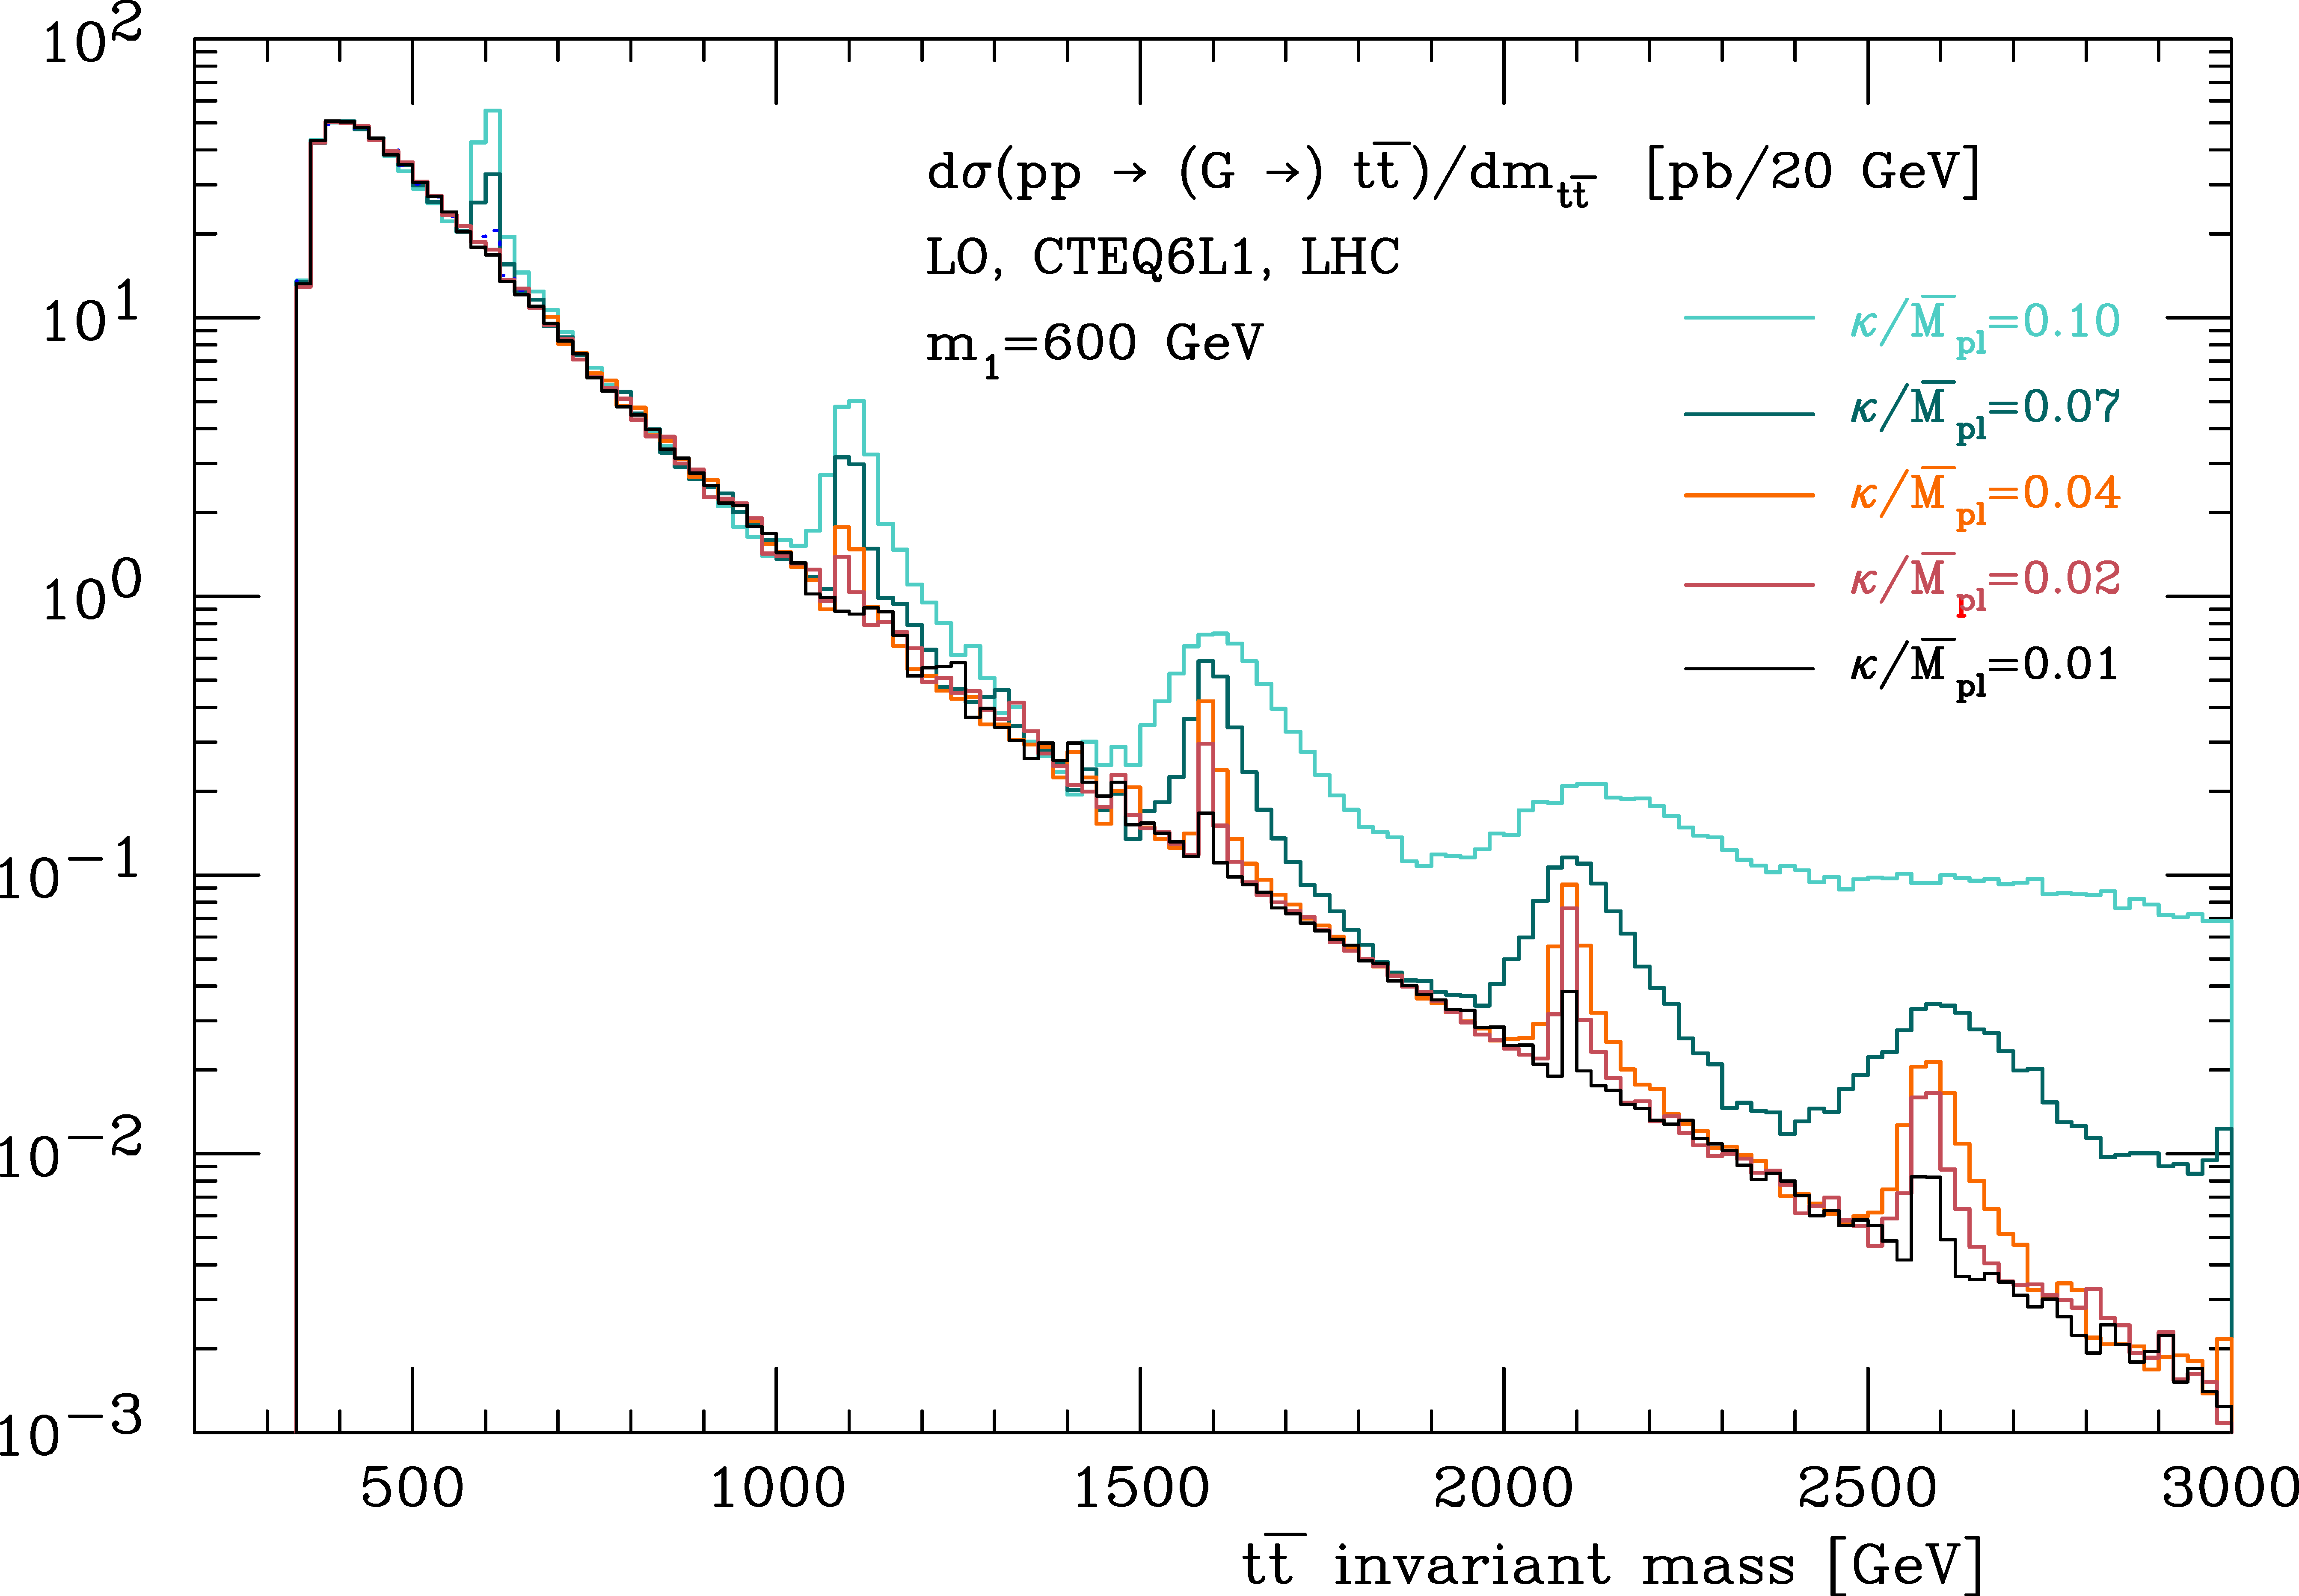
\includegraphics[width=0.60\textwidth]{chapitre5/figs/mtt_gravitons_RS.pdf}
    \caption{Distribution de masse invariante \ttbar en présence de résonances de gravitons de Kaluza-Klein, prédites par le modèle Randall-Sundrum. La masse du premier mode d'excitation est $m = \SI{600}{\GeV}$, et les différentes couleurs représentes différents choix de paramètres théoriques \citep{Frederix:2007gi}.}
    \label{fig:mtt_gravitons_RS}
\end{figure}

Une extension courante des modèles de Randall-Sundrum \citep{Davoudiasl:2000wi,Lillie:2007yh,Agashe:2003zs,Agashe:2006hk} permet en plus d'expliquer la hiérarchie de masses entre les particules du Modèle Standard. Dans ces modèles, les champs du Modèle Standard sont autorisés à se propager dans la dimension supplémentaire. Comme la dimension est compactifiée, on voit apparaitre des excitations de Kaluza-Klein pour tous les fermions et bosons du Modèle Standard. On identifie ainsi les particules du Modèle Standard comme étant les excitations d'ordre 0 de Kaluza-Klein.
Les fermions acquièrent leur masse grâce au couplage avec le champ de Higgs. La masse "4d" est obtenue en intégrant le long de la \ordinalnum{5} dimension :
\begin{align*}
  m_i &\propto \int \limits_{-\pi R}^{\pi R} \frac{\mathrm{d}y}{2 \pi R} \, \lambda_i^\text{(5)} \, e^{-4 \kappa \abs{y}} \, H(y) \, f_0^i(y) \\
  H(y) &= H_0 \, e^{4 \kappa \left(\abs{y} - \pi R \right)}
\end{align*}
où $i$ représente le fermion considéré (\Pe, \Pmu, \Ptop, ...), $\lambda_i^\text{(5)}$ le couplage de Yukawa "5d", $H(y)$ est la fonction d'onde dans la \ordinalnum{5} dimension associée au boson de Higgs et $f_0^i(y)$ la fonction d'onde dans la \ordinalnum{5} dimension associée au fermion $i$. Ainsi, la masse des fermions dépend du recouvrement entre les deux fonctions d'ondes. En supposant que la fonction d'onde du Higgs est quasiment localisée sur la brane \si{\TeV} (voir \cref{fig:rs}, en \gris), il est possible d'expliquer la hiérarchie des masses en choisissant judicieusement les fonctions d'ondes associées aux fermions : plus le recouvrement avec la fonction d'onde du Higgs sera grand, plus la masse du fermion sera importante. Par exemple, pour expliquer la grande masse du quark top, on privilégiera une fonction d'onde ayant un fort recouvrement (courbe \rouge sur la \cref{fig:rs}), et pour les autres fermions, un faible recouvrement (courbe \orange sur la \cref{fig:rs}).

\medskip

\begin{figure}[tbp]
    \centering
    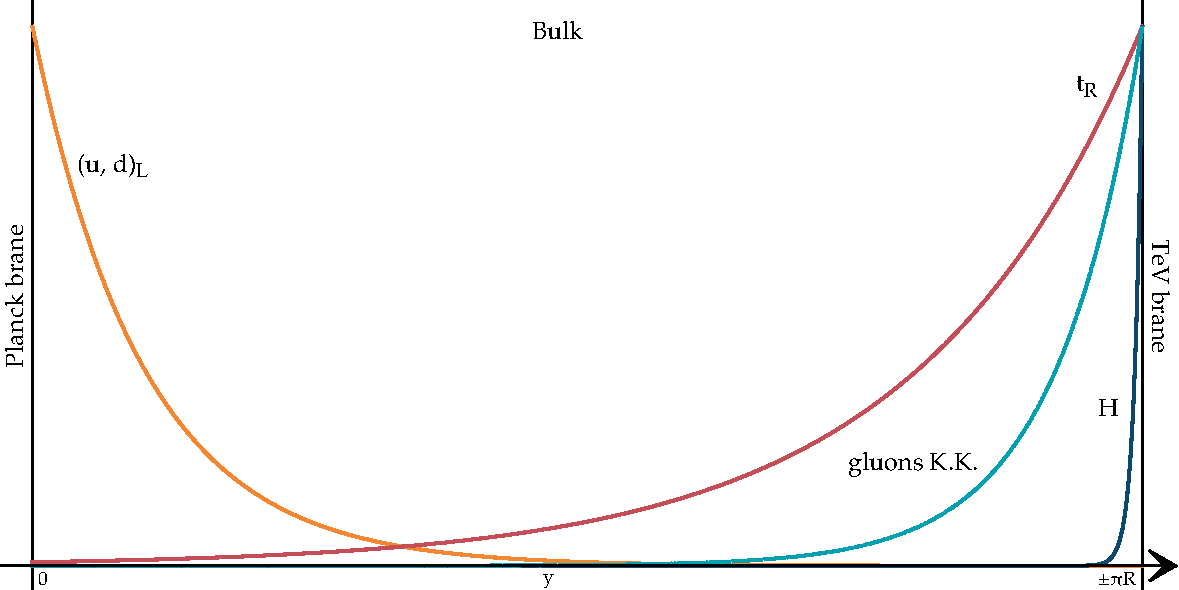
\includegraphics[width=0.8\textwidth]{chapitre5/figs/RS/RS_wave_functions.pdf}
    \caption{Représentation schématique des fonctions d'ondes dans la \protect\ordinalnum{5} dimension.}
    \label{fig:rs}
\end{figure}

Parmi les signatures expérimentales de ces modèles, attardons nous spécifiquement sur le premier mode excité des gluons, un gluon massif de spin 1 (\kkg, \kkglu). Du fait du très fort recouvrement entre les fonctions d'ondes des quarks top et des gluons K. K. (voir \cref{fig:rs}), la rapport d'embranchement $\kkg \rightarrow \ttbar$ est proche de \SI{100}{\percent}. L'étude du spectre de masse \ttbar est alors le moyen le plus prometteur de mettre en évidence de telles particules.

\section{Conclusion}

On a vu au travers ce chapitre que les propriétés du quark top sont encore assez mal connues, tout du moins avec une précision moindre que les autres particules du Modèle Standard. Néanmoins, de nombreuses études sont menées afin d'améliorer nos connaissances, indispensables pour la recherche de nouvelle physique, mais également pour vérifier la cohérence du Modèle Standard.

\medskip

De nombreuses extensions du Modèle Standard prédisent de nouvelles particules se désintégrant préférentiellement en quark top. Expérimentalement, ces particules peuvent se manifester par la présence de résonances dans le spectre de masse \ttbar. Suivant le spin et le mode de production des particules, ces résonances peuvent avoir des structures différentes, comme un pic dans le spectre de masse, voire des structures plus compliquées comme un pic - trou. Il est donc primordial d'avoir une excellente connaissance de \mtt pour espérer détecter des déviations.

\smallskip

L'étude du spectre de masse \mtt est donc un puissant moyen de recherche de nouvelle physique : les \cref{chap:zprime,chap:higgs} exploitent ainsi \mtt pour la recherche expérimentale de nouvelle physique : le \cref{chap:zprime} sera consacré à la recherche de résonances de spin 1, telles que prédites par les modèles topcolor et Randall-Sundrum. Le \cref{chap:higgs} sera lui consacré à la recherche de résonances de spin 0, telles que prédites par les modèles à deux doublets de Higgs.

\end{fmffile}